\chapter{Results and Discussion}
\label{chapter: results and discussion}

In this chapter, I will present and discuss the results gained from spectra produced and analyzed by the self-developed code \textit{AXAWOTLS}. I will organize the results into three categories:

\begin{enumerate}
	\item \textbf{Qualitative Performance:} The results in this category serve to 
	assess the spectrometers qualitatively and to touch on the properties 
	of the laser-driven backlighters. The fundamental 
	outputs of the spectrometers will be presented, which take the form of source 
	spectra of various backlighter targets as well as absorption spectra of cold 
	aluminum, where here cold refers to ambient vacuum temperatures.
	\item \textbf{Spectrometer Characterization:} This covers the quantitative characterization of the spectrometers, consisting of the calculation of the spectral resolution through two spectral 
	features: the He-$\upalpha$ line (corresponding to the n=2 to n=1 transition of 
	He-like ions, starting from 2p$^1$P$_1$) of aluminum in source spectra 
	and the Al 
	K-edge in transmission spectra. Additionally, the ratio of integrated 
	reflectivities of both spectrometers for a given event will be determined. To note is that the 
	integrated reflectivity itself cannot be directly determined, as the total 
	emission of the x-ray sources are unknown.
	\item \textbf{Setup Validation:} The purpose of this category is to check that 
	the experimental setup yields plausible results considering the characteristics of the x-ray sources. To this end the conversion efficiency 
	of the laser energy into the Al He-$\upalpha$ emission is determined, serving as a quantitative validation through comparison to literature.
\end{enumerate}

In light of the results, the effectiveness of each spectrometer design in the context of this work will be discussed. I will then use these considerations to inform a recommended spectrometer design for future experiments.

I will begin with the qualitative performance, which will be 
prefaced by a brief introduction to the main mechanisms of X-ray emission from laser-generated plasmas, since 
it is important for the discussion of the source and absorption spectra. This 
will be followed by the spectrometer characterization and setup validation. For each set of results, I will first explain the processing steps, then present the results, and end with a discussion detailing the ramifications for the spectrometer designs. In addition, the error calculations will be described in the appendix chapter \ref{chapter: uncertainty analysis}.

\section{Qualitative Performance}
\label{section: qualitative performance}

As stated in the spectrometer comparison of section \ref{section: specs and comparison}, neither the DUCC nor the FSSR-1D clearly distinguishes itself from design specifications, e.g. in terms of theoretical relative resolution and sample size. As such, the qualitative assessment of the performance of each spectrometer during the experiment plays an important role. The most significant results in this area are of course the absorption spectra, whose quality depends on a number of experimental factors and mechanical properties, e.g. crystal quality, backlighter type, accuracy of the alignment of the setup, etc. To understand the details of the XAFS spectra quality, it is necessary to first study the spectra of the x-ray sources, i.e. the laser-driven plasma emission. Accordingly, I will begin by summarizing the main x-ray emission mechanisms in laser-driven plasma, then present source spectra.


\subsection{X-ray Source Spectra}

There are three main mechanisms responsible for
x-ray emission in laser-generated plasma, each identifiable by their characteristics on the spectrum \citep{riley2021warm, 
	giulietti1998x}. The first originates from scattering of free electrons with 
ions in the plasma. This generates bremsstrahlung and 
gives a smooth emission spectrum, where the intensity
decreases for increasing photon energy. As this 
emission depends on average ionization, it is 
strongest for high Z materials. The second is 
recombination, in which free electrons recombine with 
ions and radiate a photon. This also results in a 
continuous spectrum, but deviates from bremsstrahlung emission in that it occurs from a minimum photon energy 
called the recombination edge. These edges also 
result in jumps in the spectrum corresponding to 
recombination stages. The third is line emission, 
occurring for transitions of bound electrons between 
states. This is the strongest source of x-ray 
radiation in terms of photons per energy interval, but is also discrete \citep{giulietti1998x}. 

Based on these different kinds of x-ray emission mechanisms, the characteristics of x-ray backlighters can be tailored to their application. An ideal x-ray source for XAFS would exhibit a high-intensity, spectrally quasi-continuous spectrum, as this reduces the chance of spectral structure, like peaks or edges, impacting the absorption spectrum, as well as ensures good signal-to-noise ratios \citep{riley2021warm, eason1984improved}. In practice, continuum x-ray emission is usually realized by plasma of either very low-Z or high-Z ($\geq$20) material. In the case of very low-Z targets, ions are fully stripped, thus suppressing line emission so that Bremsstrahlung dominates. For high-Z targets, the spectrum is dominated by line emissions from many-electron interactions, leading to a high line density and therefore a quasi-continuous spectrum. As such, very low-Z targets offer smooth spectra at the cost of having low intensity, while high-Z backlighters yield high intensities with potential significant structure in the spectrum \citep{giulietti1998x}.

In light of this, five high-Z elements are tested in this experiment, namely gold and four rare earth elements: samarium, 
gadolinium, terbium, and dysprosium. Additionally, a low-Z material is investigated in the form of Teflon. Figure \ref{figure: basic spectra} depicts source spectra for each backlighter material as well as aluminum, a material used for spectrometer characterization and as a control. The spectra are all extracted and processed according to the procedure described in chapter \ref{chapter: data analysis}. When available, events with different laser energies are shown. All the source spectra, excepting those of Teflon, are captured with the DUCC, as it simultaneously displays the fewest spectral artefacts, often originating from crystal defects or damage, and good resolution, as will be demonstrated in section \ref{subsection: spectral resolution}. Owing to the lower intensity of the emission as compared to the high-Z elements, the Teflon source spectra are taken with the SUCC, whose KAP crystal has a higher integrated reflectivity. The greater collection rate of the SUCC is demonstrated in fig. \ref{fig: Al DUCC series}, where approximately three times more photons land on the detector (filter corrected) as compared to the DUCC. 

\begin{figure} [H]
	\centering
	\begin{subfigure}[t]{0.49\textwidth}
		\centering
		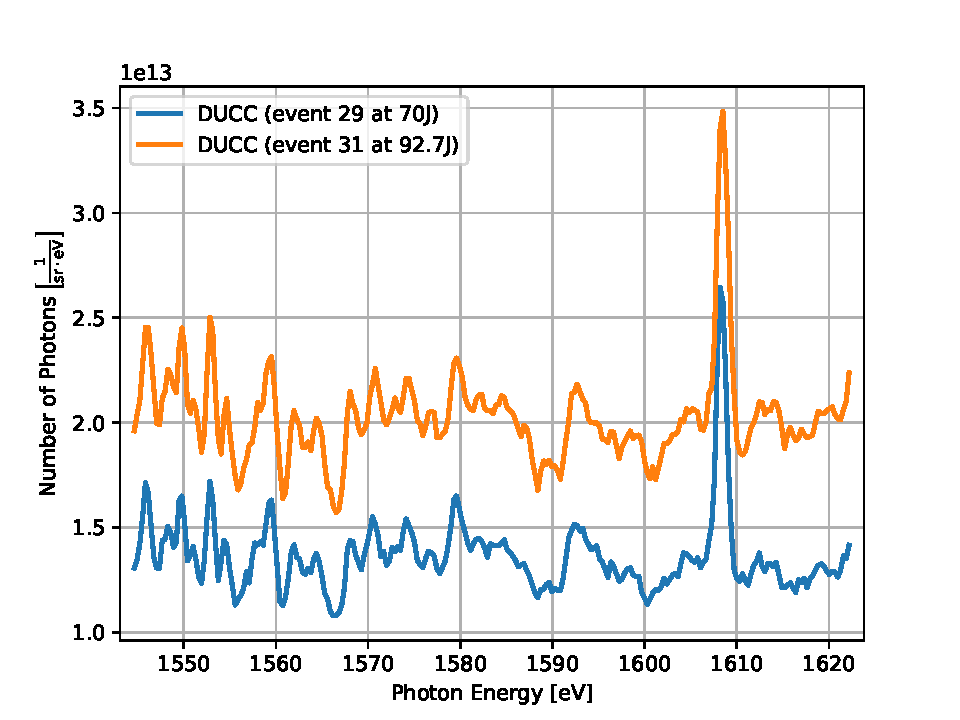
\includegraphics[width=\textwidth]{Data_Analysis/basic_spectra/spectra_of_Sm_events_29_31.pdf}
		\caption{Source spectra of samarium detected with the DUCC.}
		\label{}
	\end{subfigure}%
	\hfill
	\begin{subfigure}[t]{0.49\textwidth}
		\centering
		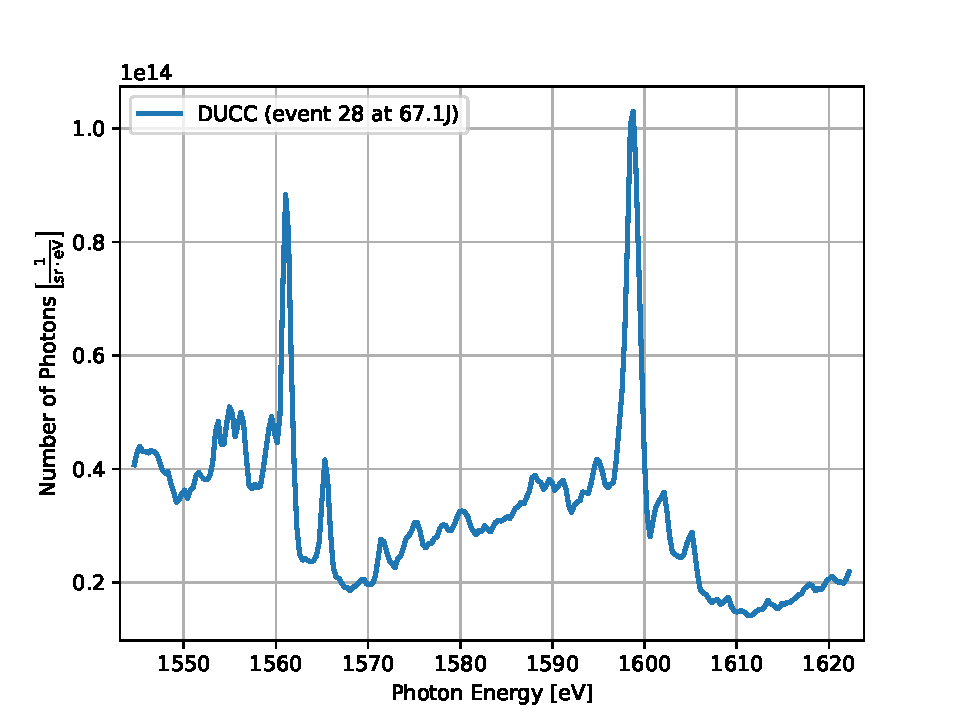
\includegraphics[width=\textwidth]{Data_Analysis/basic_spectra/basic_spectrum_of_Tb_event_28_on_DUCC.pdf}
		\caption{Source spectrum of terbium detected with the DUCC.}
		\label{}
	\end{subfigure}
	\begin{subfigure}[t]{0.49\textwidth}
		\centering
		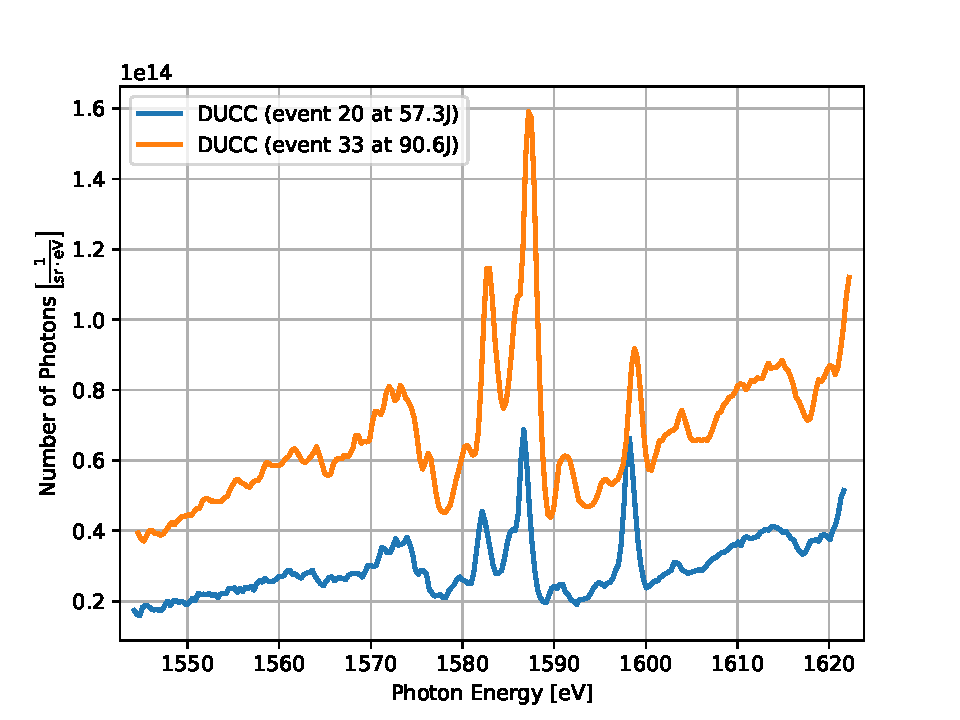
\includegraphics[width=\textwidth]{Data_Analysis/basic_spectra/spectra_of_Dy_events_20_33.pdf}
		\caption{Source spectra of dysprosium detected with the DUCC.}
		\label{}
	\end{subfigure}%
	\hfill
	\begin{subfigure}[t]{0.49\textwidth}
		\centering
		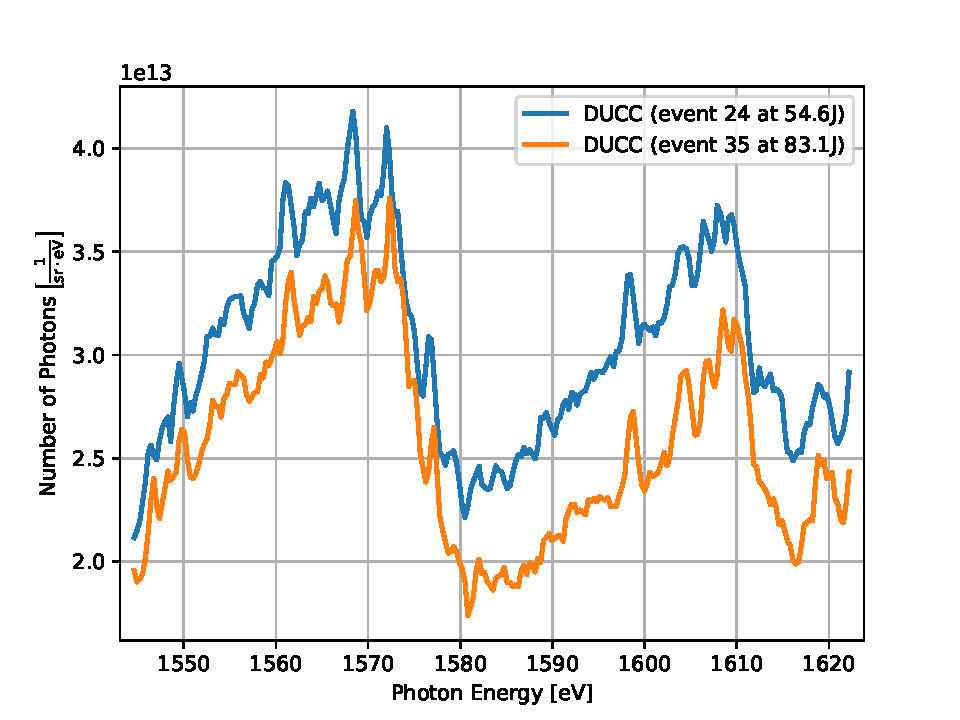
\includegraphics[width=\textwidth]{Data_Analysis/basic_spectra/spectra_of_Gd_events_24_35.pdf}
		\caption{Source spectra of gadolinium detected with the DUCC.}
		\label{}
	\end{subfigure}
	\begin{subfigure}[t]{0.49\textwidth}
		\centering
		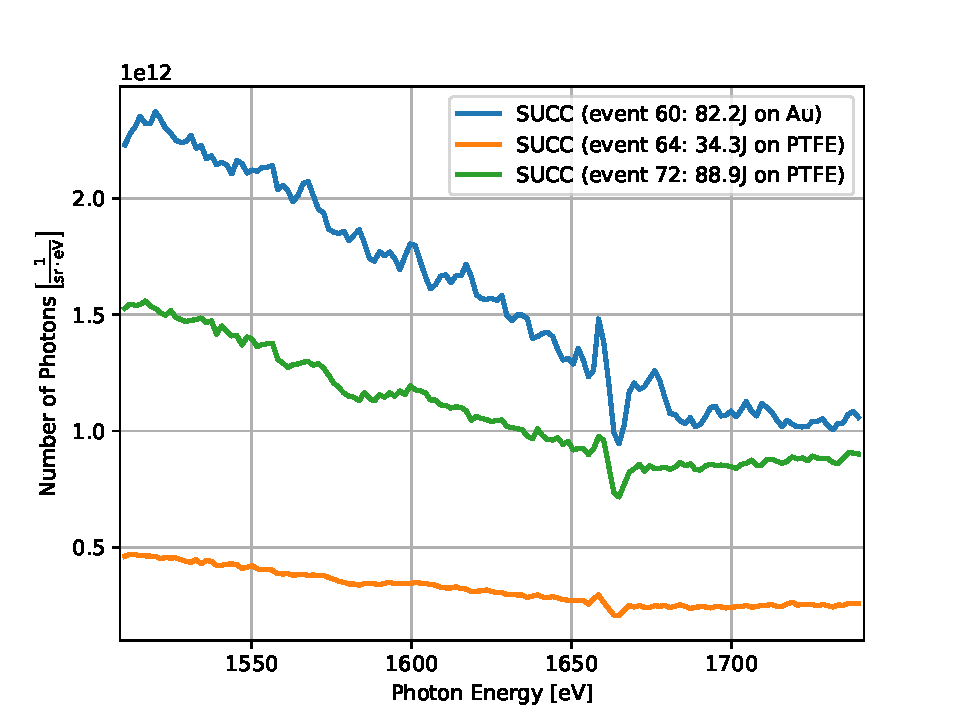
\includegraphics[width=\textwidth]{Data_Analysis/basic_spectra/spectra_of_PTFE_events_60_64_72.pdf}
		\caption{Source spectra of Teflon (PTFE) and gold detected with the SUCC.}
		\label{subfigure: PTFE basic spectra}
	\end{subfigure}%
	\hfill
	\begin{subfigure}[t]{0.49\textwidth}
		\centering
		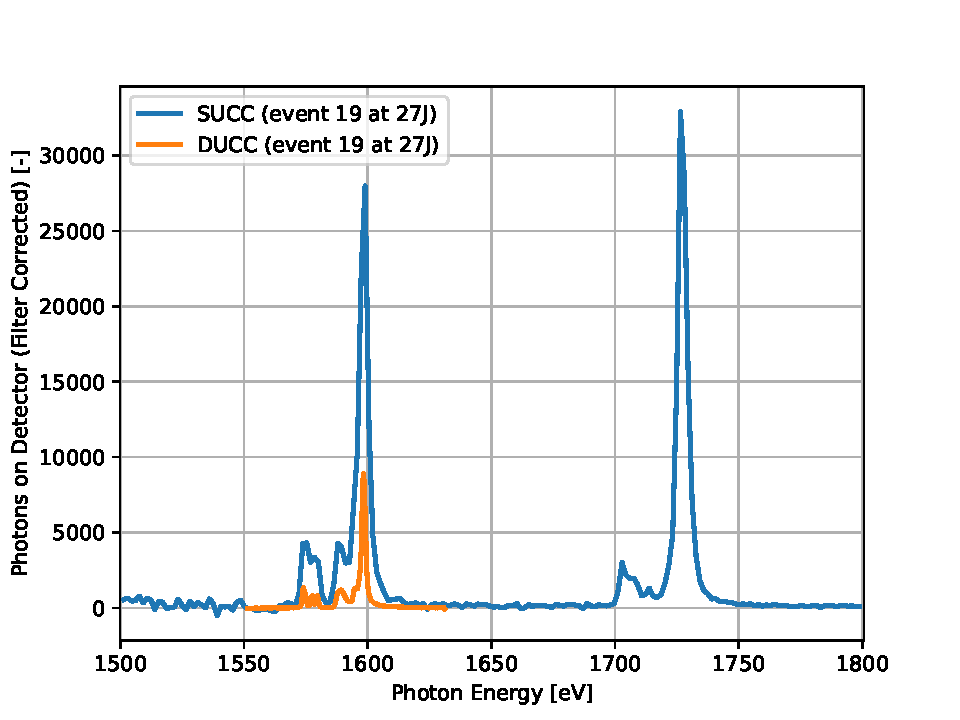
\includegraphics[width=\textwidth]{Data_Analysis/basic_spectra/spectra_of_Al_events_19_19.pdf}
		\caption{Source spectrum of aluminum detected with the DUCC and SUCC respectively.}
		\label{fig: Al DUCC series}
	\end{subfigure}
	\caption{Source spectra of laser-driven plasma from various backlighter materials. Shots of different laser energies are shown when available. Notably, the Teflon spectra are from the SUCC because the signal-to-noise ratio for the DUCC is in this case poor, as the intensity of the emission is at least an order of magnitude lower than for other backlighters.}
	\label{figure: basic spectra}
\end{figure}

In general, the spectrometers successfully produce results qualitatively in agreement with the expected source spectra. Each rare earth spectrum is dominated by high density line emission, recognizable in the peak-heavy structures, whereas the Teflon and gold spectra exhibit a quasi-continuous spectrum whose intensity falls with increasing photon energy, as is consistent with recombination or bremsstrahlung emission. Additionally, for backlighter materials with shots of various laser energies (see fig. \ref{figure: basic spectra}) the emission is stronger for greater laser energy, with the exception of gadolinium, where the \SI{54.6}{\joule} shot displays lower photon numbers than the \SI{83.1}{\joule} shot. The difference can be explained by the use of a phase plate in front of the PHELIX laser for the latter shot, which reduces the overall laser intensity. Overall, the consistency of the source spectra with expectations serves as a first validation of the spectrum processing procedure and the efficacy of the spectrometers.

\begin{figure} [H]
	\centering
	\begin{subfigure}[t]{0.7\textwidth}
		\centering
		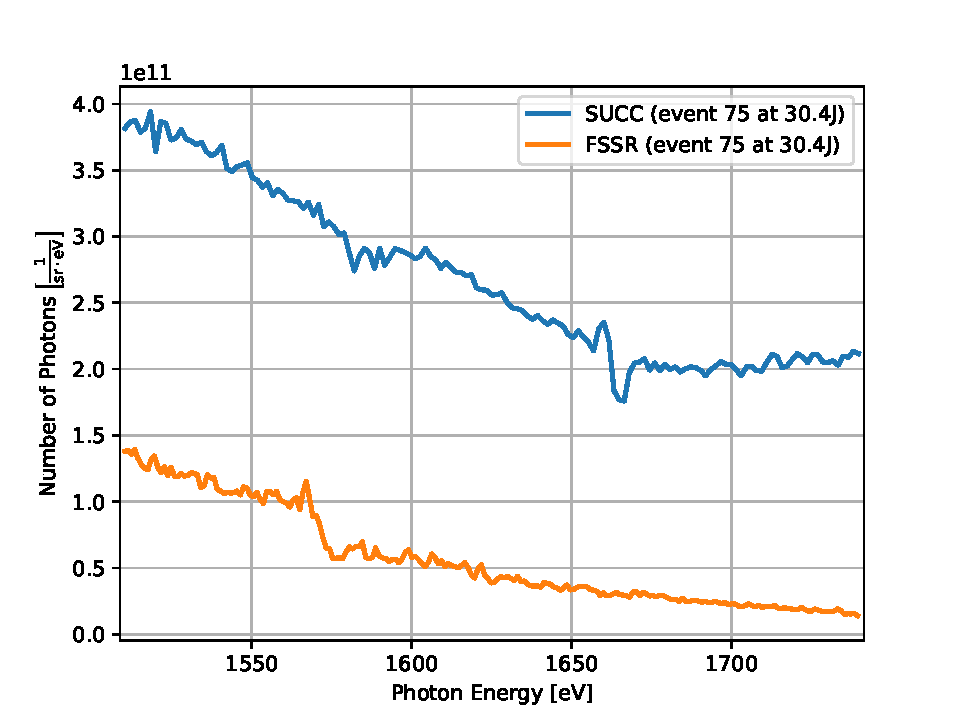
\includegraphics[width=\textwidth]{Data_Analysis/basic_spectra/spectra_of_PTFE_events_75_75.pdf}
		\caption{Source spectrum of Teflon detected with the FSSR and SUCC respectively.}
		\label{fig: FSSR basic spectrum}
	\end{subfigure}
	\hfill
	\begin{subfigure}[t]{\textwidth}
		\centering
		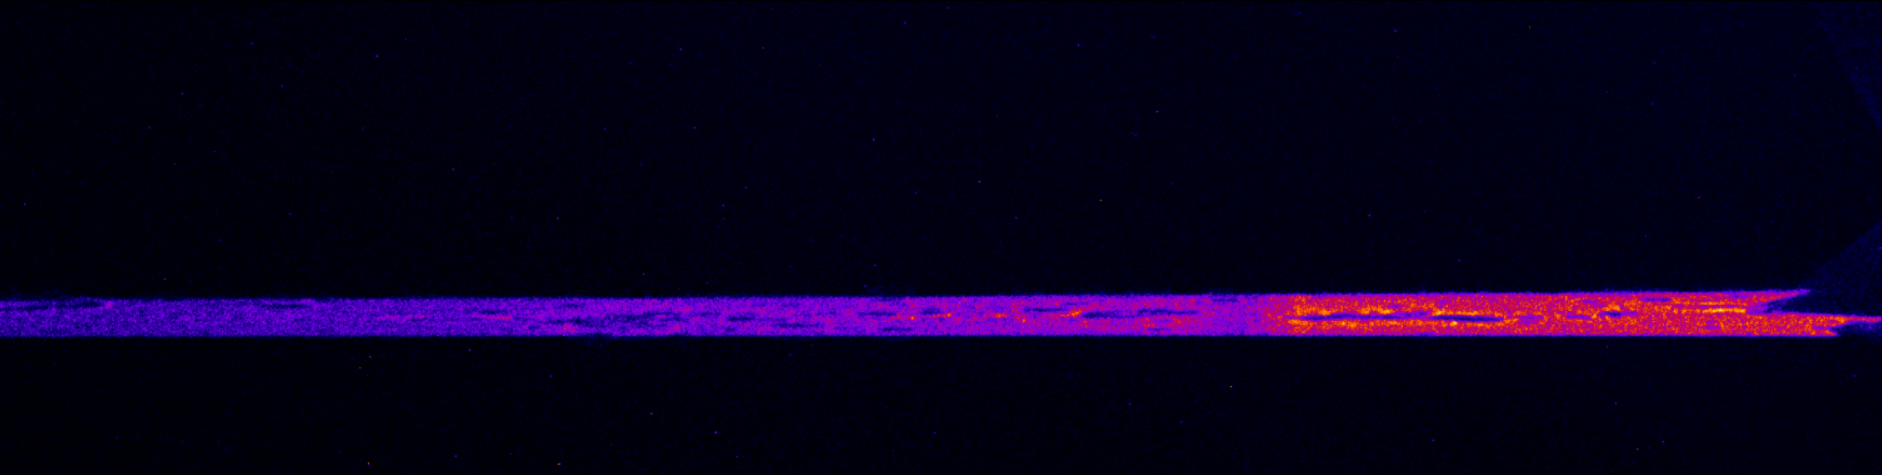
\includegraphics[width=\textwidth]{Data_Analysis/basic_spectra/FSSR_75.png}
		\caption{Raw TIFF image from the FSSR (unfocused) for a shot on Teflon at \SI{30.4}{\joule} (event 75).}
		\label{fig: FSSR TIFF}
	\end{subfigure}
	\caption{(a) shows the difference in spectra from a single shot on Teflon for different spectrometers. From this one can identify spectral features that most likely are linked to crystal defects and properties. Notable is the dip at $\approx$\SI{1570}{\electronvolt} in the spectrum from the FSSR, an artefact of the Al K-edge originating from the presence of aluminum in the mica crystal makeup. (b) is a TIFF image for the FSSR with a defocusing of \SI{5}{\milli\meter}, showing the numerous holes and deformations in the raw image of the FSSR, which are due to crystal defects and damage.}
	\label{}
\end{figure}

It is important to note that not all structures of the spectra are from the spectral properties of the emission. A significant source of spectral artefacts are the crystals, e.g. from defects in the lattice structure or outside influences, like dirt or imperfect adherence to the substrate. One example of such a spectral feature can be found in fig. \ref{subfigure: PTFE basic spectra}, where at approximately \SI{1660}{\electronvolt} there are a sudden rise and dip in all the spectra independent of the backlighter material. Such spectral features are also present and especially prevalent for the FSSR. As is apparent from fig. \ref{fig: FSSR basic spectrum}, the FSSR spectra are laden with features that are most likely caused by defects and properties of the spherically bent mica crystal, impacting the source spectrum. For example, a dip occurs for the FSSR at $\approx$\SI{1570}{\electronvolt}, preceded by a small peak at $\approx$\SI{1565}{\electronvolt}. These artefacts are likely caused by a K-edge from the aluminum component in the mica and by holes and features in the raw image (see fig. \ref{fig: FSSR TIFF}) that can be traced back to defects in the crystal. To note is that for a standard FSSR-1D setup, the signal would appear as a single horizontal line. In this case, the image was unfocused by extending the crystal-detector distance $b_0$ by \SI{5}{\milli\meter}, shifting the detector away from the Rowland circle.  Besides the difficulties of the crystal quality, the FSSR performed qualitatively as designed in that the predicted focusing properties were successfully reproduced and that spectra with the expected dispersion were extracted.

\subsection{X-ray Absorption Spectra}
\label{subsection: ab spectra}

The processing of the x-ray absorption spectra begins with the extraction of the spectra for a given absorption shot analogously to the previous section, yielding a source and transmitted spectrum from the same x-ray source. The two spectra are then aligned with an algorithm that shifts the source spectrum until the best possible alignment is found in a given energy range; a step made necessary by small shot-to-shot deviations of the x-ray source position. Once aligned, the photon energy dependent transmission $T(E)$ is calculated by the ratio of the transmitted intensity $I_{trans}$ to the source spectrum intensity $I_{source}$. The absorption coefficient $\mu$ can then be determined with the equation 
\begin{equation}
	\mu = \frac{-\ln(T)}{d_{Al,eff}},
\end{equation}
where the effective aluminum thickness $d_{Al,eff}$ takes into account the angle of the x-rays to the sample surface. The sample material was provided with an error of 10\% for $d_{Al}$, which gets passed onto the absorption coefficient using Gaussian error propagation.

While this procedure is effective for crystals of excellent quality, the processing can be improved by including a crystal calibration step. This step consists of using a calibration shot, in which spectra without a sample are taken with ideally the same setup and laser parameters as the absorption shot, in order to account for spectral features from crystal defects. In this case, the transmission is calculated by
\begin{equation}
	T = \frac{(I_{trans}/I_{source})}{(I_{cal,trans}/I_{cal,source})},
\end{equation}
where $I_{cal,trans}$ and $I_{cal,source}$ are the calibration spectra corresponding to the spectrometers/spectrometer channels of the transmitted and source spectrum of the absorption shot. To note is that this calibration introduces further complexity to the processing and hinges on how accurately the shots are reproduced, i.e. with low fluctuation of the x-ray source position and same backlighter at similar laser energy. Accordingly, I chose to apply this crystal calibration to the OSUCC/SUCC absorption shot, since the spectrometers are not identical and the crystals were of differing quality. I did not apply this calibration to the shots with the DUCC as no suitable calibration shots exist and the ADP crystals were of relatively good quality, in that they display few noticeable spectral features.

For all the results presented, the Al sample was placed directly on the spectrometer channel entrance to ensure that the Al foil remained at ambient temperature, i.e. so that no preheating due to proximity to the backlighter occurs. The experimental results are validated by an Al absorption spectrum published by \textit{Levy et al.} \citep{levy2010double}, whose experimental setup is similar to our own with the DUCC, with the key differences that they used erbium as backlighter and conically-bent crystals for their spectrometer



\begin{figure} [!htbp]
	\centering
	\begin{subfigure}[t]{0.88\textwidth}
		\centering
		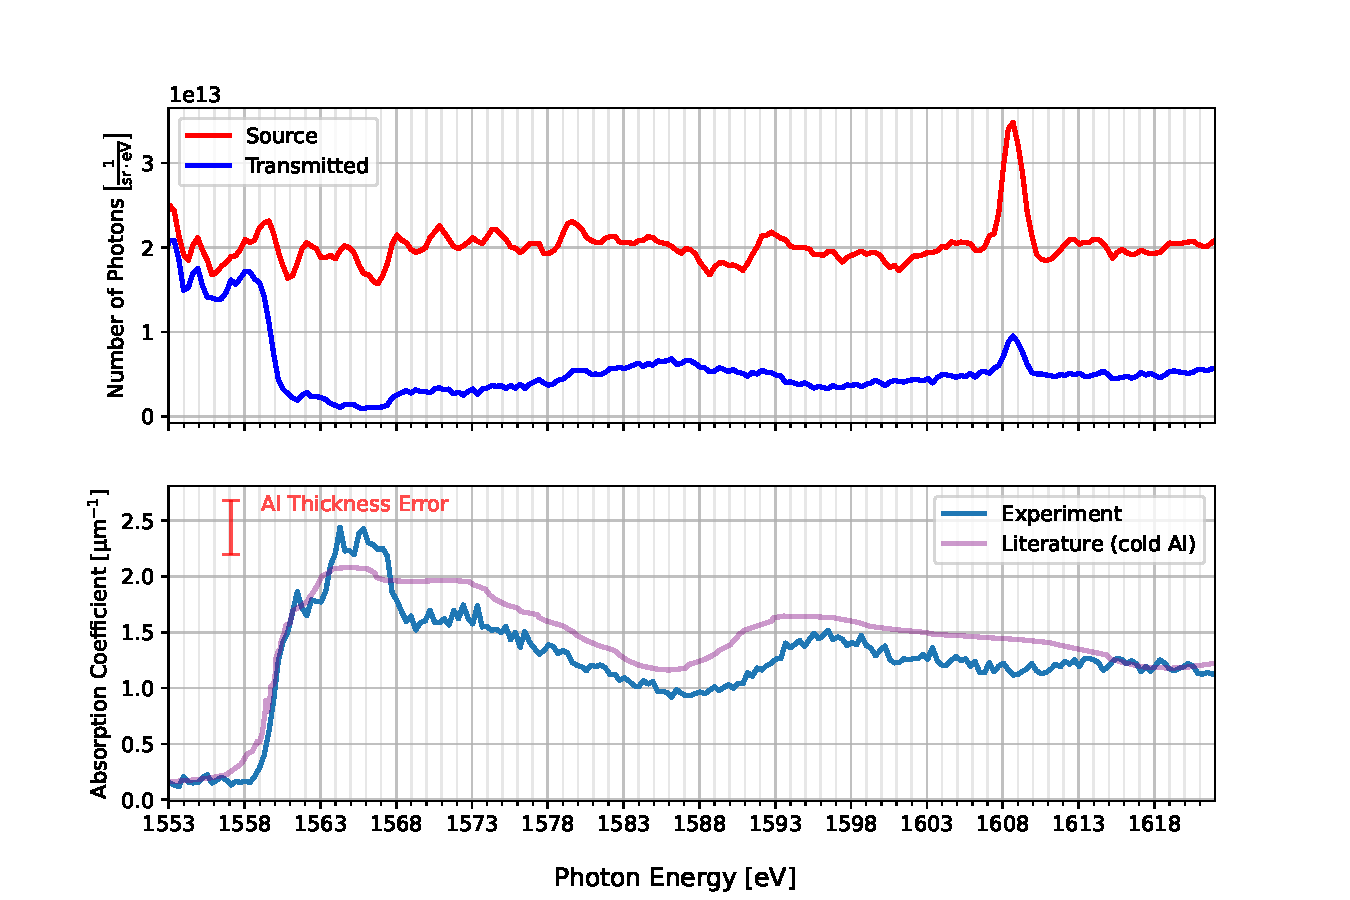
\includegraphics[width=\textwidth]{Data_Analysis/absorption_wo_calibration/absorption_spectrum_of_Sm_event_31_on_DUCC.pdf}
		\caption{X-ray absorption spectrum through a \SI{1.18\pm0.12}{\micro\meter} thick aluminum foil for a \SI{97.4}{\joule} shot on samarium.}
		\label{fig: DUCC absorption Sm}
	\end{subfigure}%
	\hfill
	\begin{subfigure}[t]{0.88\textwidth}
		\centering
		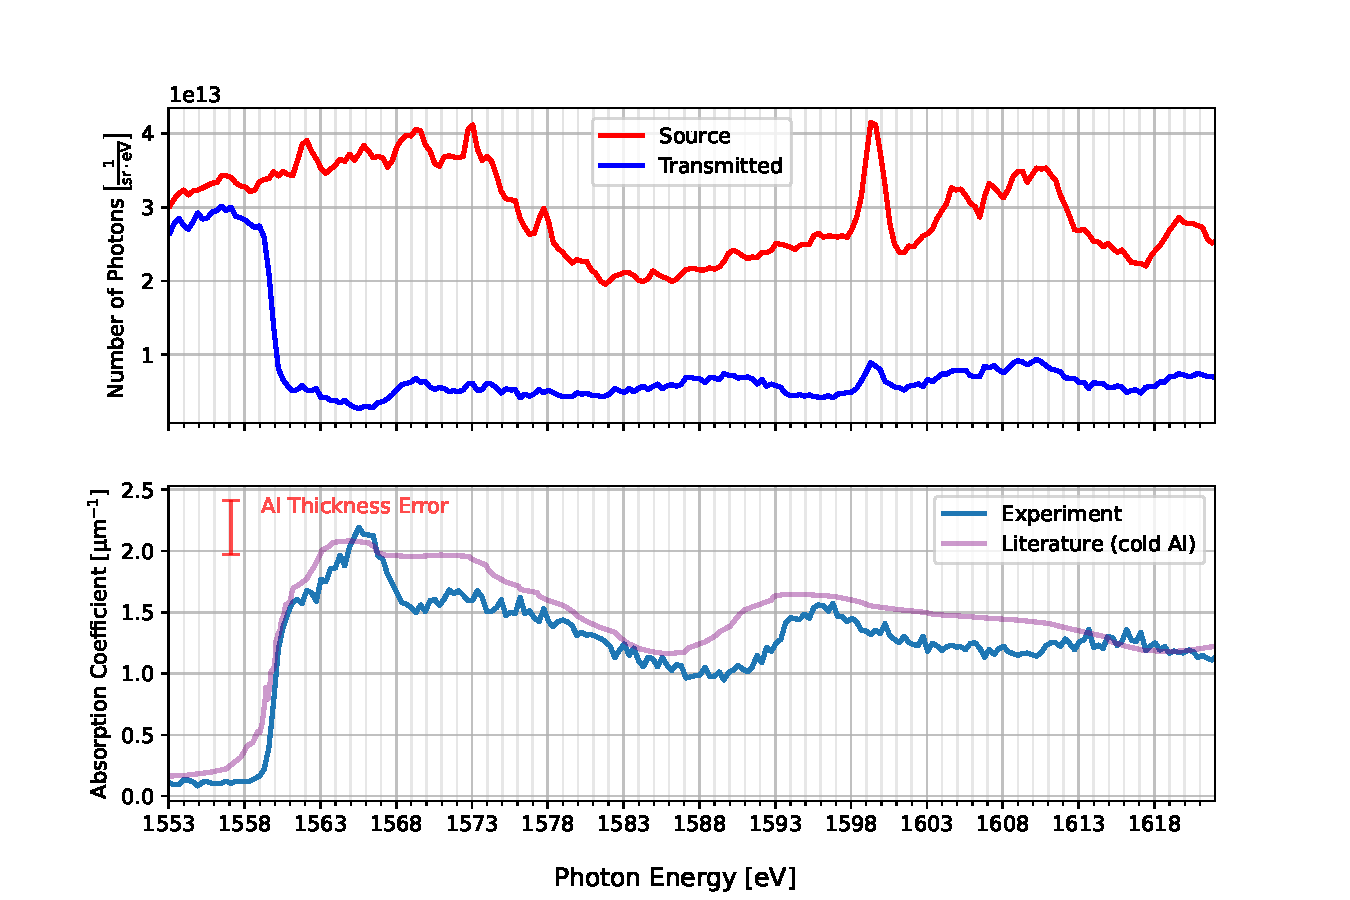
\includegraphics[width=\textwidth]{Data_Analysis/absorption_wo_calibration/absorption_spectrum_of_Gd_event_32_on_DUCC.pdf}
		\caption{X-ray absorption spectrum through a \SI{1.18\pm0.12}{\micro\meter} thick aluminum foil for a \SI{87.4}{\joule} shot on gadolinium.}
		\label{fig: DUCC absorption Gd}
	\end{subfigure}
	\caption{X-ray absorption spectra detected with the DUCC. In (a) and (b); \textbf{Top:} fully processed spectrum pair whose ratio yields the x-ray transmission through the sample. \textbf{Bottom:} absorption spectrum with comparison to a result from \textit{Levy et al.} \citep{levy2010double} and the systematic uncertainty due to the sample thickness, depicted as an error bar that aligns with the maximum value of $\mu$.}
	\label{fig: DUCC absorption}
\end{figure}

The absorption spectra of fig. \ref{fig: DUCC absorption} and \ref{fig: SUCC absorption} both exhibit reasonable agreement with the literature, with the absorption curves of the SUCC/OSUCC setup, where the first spectrometer detects the source spectrum and the second the transmitted, showing closer agreement then the spectra from the DUCC. As such, the absorption curves were successfully extracted, albeit with varying quality dependent on the spectrometer combination.

In the case of the absorption shots with the DUCC (see fig. \ref{fig: DUCC absorption}), for which the dual channels are employed to record the spectra, a reasonably good agreement with the literature curve is achieved, considering that no crystal calibration is carried out and that the transmitted and source spectra are structure-heavy. In fact, much of the structure in the absorption spectra can attributed to features of the x-ray source emission. In general, a peak in the source spectrum will yield a dip in the absorption, and vice-versa. For example, many structures occur in the range of 1561-\SI{1568}{\electronvolt} that are clearly artefacts from the source spectrum, a observation supported by the difference of the absorption curves in that range between fig. \ref{fig: DUCC absorption Sm} and fig. \ref{fig: DUCC absorption Gd}. This implies that the processing procedure for the absorption spectrum does not fully eliminate the spectral structures of the backlighter, which could be remedied by further refinement of the transmission calculation or by carrying out a crystal calibration, since the reflectivity of the two ADP crystals are likely to vary slightly depending on photon energy. Despite these deviations, the similarity of the overall behavior of the experimental absorption spectra from the DUCC, especially in the oscillation after \SI{1570}{\electronvolt}, implies qualitative consistency between shots, lending validity to the experimental setup and dual channel spectrometer design.


The two shots in fig. \ref{fig: DUCC absorption} also differ from the literature example in the magnitude of the absorption coefficient, with the experimental curve being on average lower, as well as in the dip at \SI{1568}{\electronvolt} and the location of the second peak of the oscillation at \SI{1593}{\electronvolt}. The error due to the Al sample thickness could explain the former difference. For the latter, the extra dip at \SI{1568}{\electronvolt} in the experimental absorption curve is likely due to the influence of sample thickness on XANES structures, which is illustrated in fig. 6 of the paper from \textit{Levy et al.} \citep{levy2010double}. This idea is further supported by the closer agreement of the absorption spectrum detected with the SUCC/OSUCC (see fig. \ref{fig: SUCC absorption}), where the geometry leads to a smaller effective sample thickness of \SI{0.84\pm0.08}{\micro\meter}. On the other hand, the different location of the second oscillation peak at \SI{1593}{\electronvolt} could be explained by differences in experimental setup, e.g. in the x-ray source or sample, as the deviation between the literature and experimental curve appears in all shots. The cause of both the differences should be investigated by further literature research and comparison to Al absorption curves of other experiments.

\begin{figure}[!htbp]
	\centering
	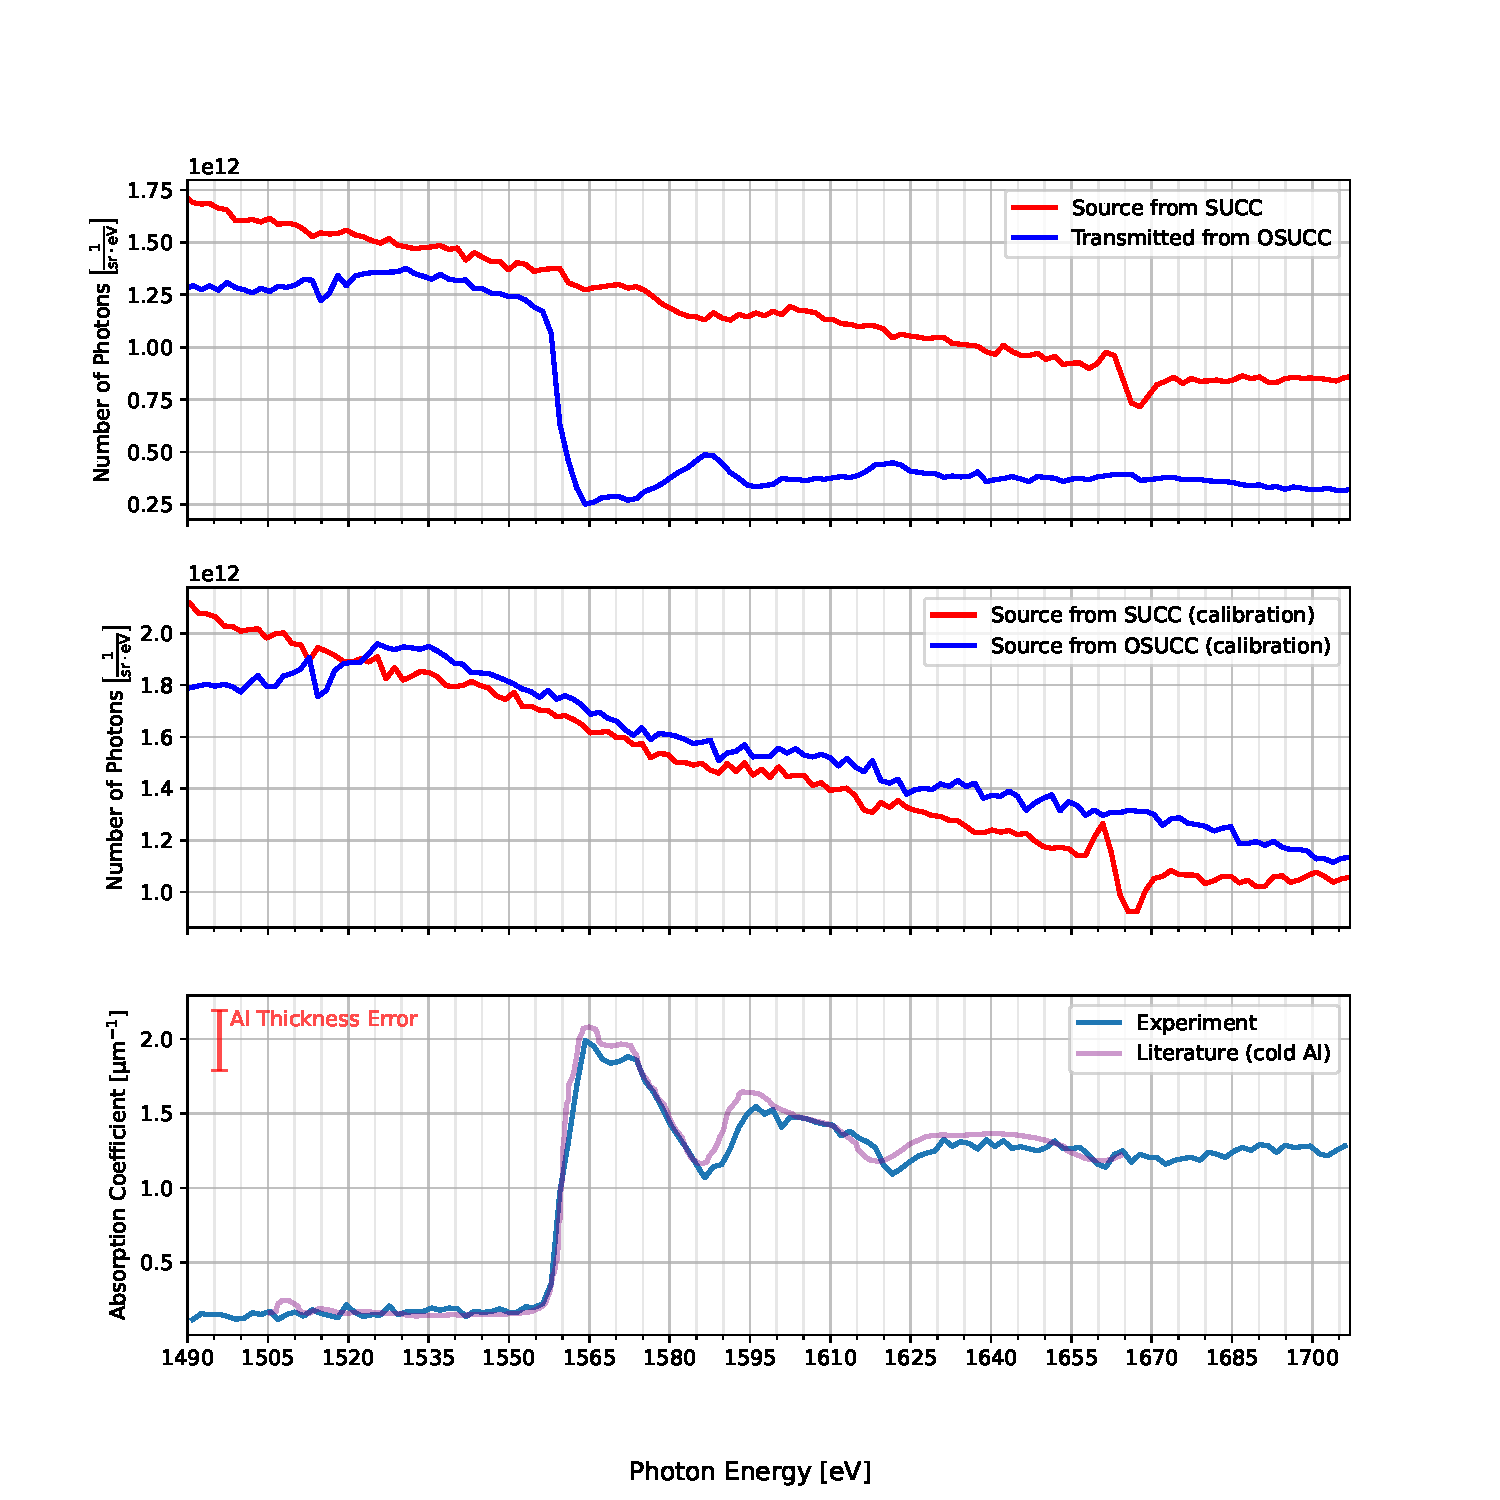
\includegraphics[width=\textwidth]{Data_Analysis/absorption/absorption_spectrum_of_PTFE_event_72_on_OSUCC.pdf}
	\caption{X-ray absorption spectrum detected with the SUCC for the source and the OSUCC for the transmitted spectrum. The crystal spectral features are corrected out using a calibration shot without a sample. \textbf{Top:} fully processed spectrum pair from a \SI{88.9}{\joule} shot on Teflon. The ratio of transmitted to source spectrum along with the crystal calibration yields the x-ray transmission through a \SI{0.84\pm0.08}{\micro\meter} thick aluminum foil sample. \textbf{Middle:} fully processed calibration spectrum pair from a \SI{110.3}{\joule} shot on Teflon. \textbf{Bottom:} absorption spectrum with comparison to a result from \textit{Levy et al.} \citep{levy2010double} and the systematic uncertainty due to the sample thickness, depicted as an error bar that aligns with the maximum value of $\mu$.}
	\label{fig: SUCC absorption}
\end{figure}

In contrast to the DUCC, the absorption spectrum pictured in fig. \ref{fig: SUCC absorption} is extracted using two separate single channel spectrometers, namely the SUCC and OSUCC, and a Teflon backlighter, which displays an exceptionally smooth x-ray source spectrum. Interestingly, the resulting absorption curve shows overall excellent agreement with the literature except for slight deviations of a few eV for the oscillation's peaks and valleys after \SI{1580}{\electronvolt}, which could be explained by experimental setup differences analogously to the discussion of the DUCC's second peak. The agreement occurs despite the fact that the KAP crystal of the OSUCC was of visibly low quality, especially apparent in the calibration spectra below \SI{1530}{\electronvolt}, and that the spectral resolutions are by nature of the spectrometer geometries different. I attribute the effectiveness of the setup to three considerations. First, the crystal features in the recorded spectra are for the most part corrected out by the crystal calibration, as apparent in the disappearance of the peak and valley around \SI{1665}{\electronvolt} inherent in both the calibration and source spectrum of the SUCC. Second, the smoothness of the Teflon spectra suppresses the difference of spectral resolutions, while reducing overall foreign structure in the absorption curve. Third, the OSUCC crystal's strongest spectral features, visible in the calibration spectrum of the OSUCC, occur below the K-edge, such that they have no influence on the fine-structures on the absorption curve. Therefore, the resulting quality of the experimental absorption spectrum demonstrates the power of a smooth backlighter spectrum as well as the crystal calibration method.

The spectrometer combination employing the SUCC/FSSR was unsuccessful, where an example with a teflon backlighter is shown in fig. \ref{fig: FSSR absorption}. Despite many attempts at tuning the alignment algorithm and selecting a suitable combination of absorption and calibration shots, the absorption spectra derived from the SUCC/FSSR setup yielded no curves that clearly aligned with that of aluminum. The main reasons are twofold. On one hand, the poor quality of the mica crystal and presence of Al in the chemical makeup lead to significant spectral structure around the K-edge energy, heavily distorting the absorption curve, especially at the edge. On the other, the vastly different geometries and function of the FSSR and SUCC hindered the aligning of the component spectra and prevented the removal of spectral structures in the absorption curve, which is most noticeable at large peaks in the backlighter emission, excluding the use of rare-earth backlighters. The difference in spectral resolution has the largest impact in this regard. Even for Teflon backlighters, the absorption spectra were not successfully extracted with the SUCC/FSSR combination (see fig. \ref{fig: FSSR absorption}). This result reflects the importance of good crystal quality, even with a meaningful tool like the crystal calibration, and similarity of the spectrometer geometries.

In summary, high quality absorption spectra are successfully extracted by the DUCC with rare-earth backlighters and the SUCC/OSUCC with Teflon, where the latter combination is closer to the literature. The SUCC/FSSR spectrometer combination does not yield viable absorption curves, even with Teflon backlighters. Accordingly, using the same spectrometers for both the source and transmitted spectra is desirable, meaning that the DUCC geometry represents the most promising setup. Additionally, the flat crystals are capable of producing low-noise, well resolved absorption spectra, as demonstrated by both the ADP crystals of the DUCC and the KAP of the SUCC/OSUCC. A smooth backlighter spectrum is also important for the quality of the absorption curves, since it simplifies processing and smooths the final absorption spectra, though the chosen x-ray source must suit the crystal, as shown by the incompatibility of Teflon backlighters with ADP. As such, combining the DUCC geometry with KAP crystals presents a promising solution, enabling the use of Teflon backlighters as well as identical geometries for the source and transmitted spectra.


\begin{figure}[H]
	\centering
	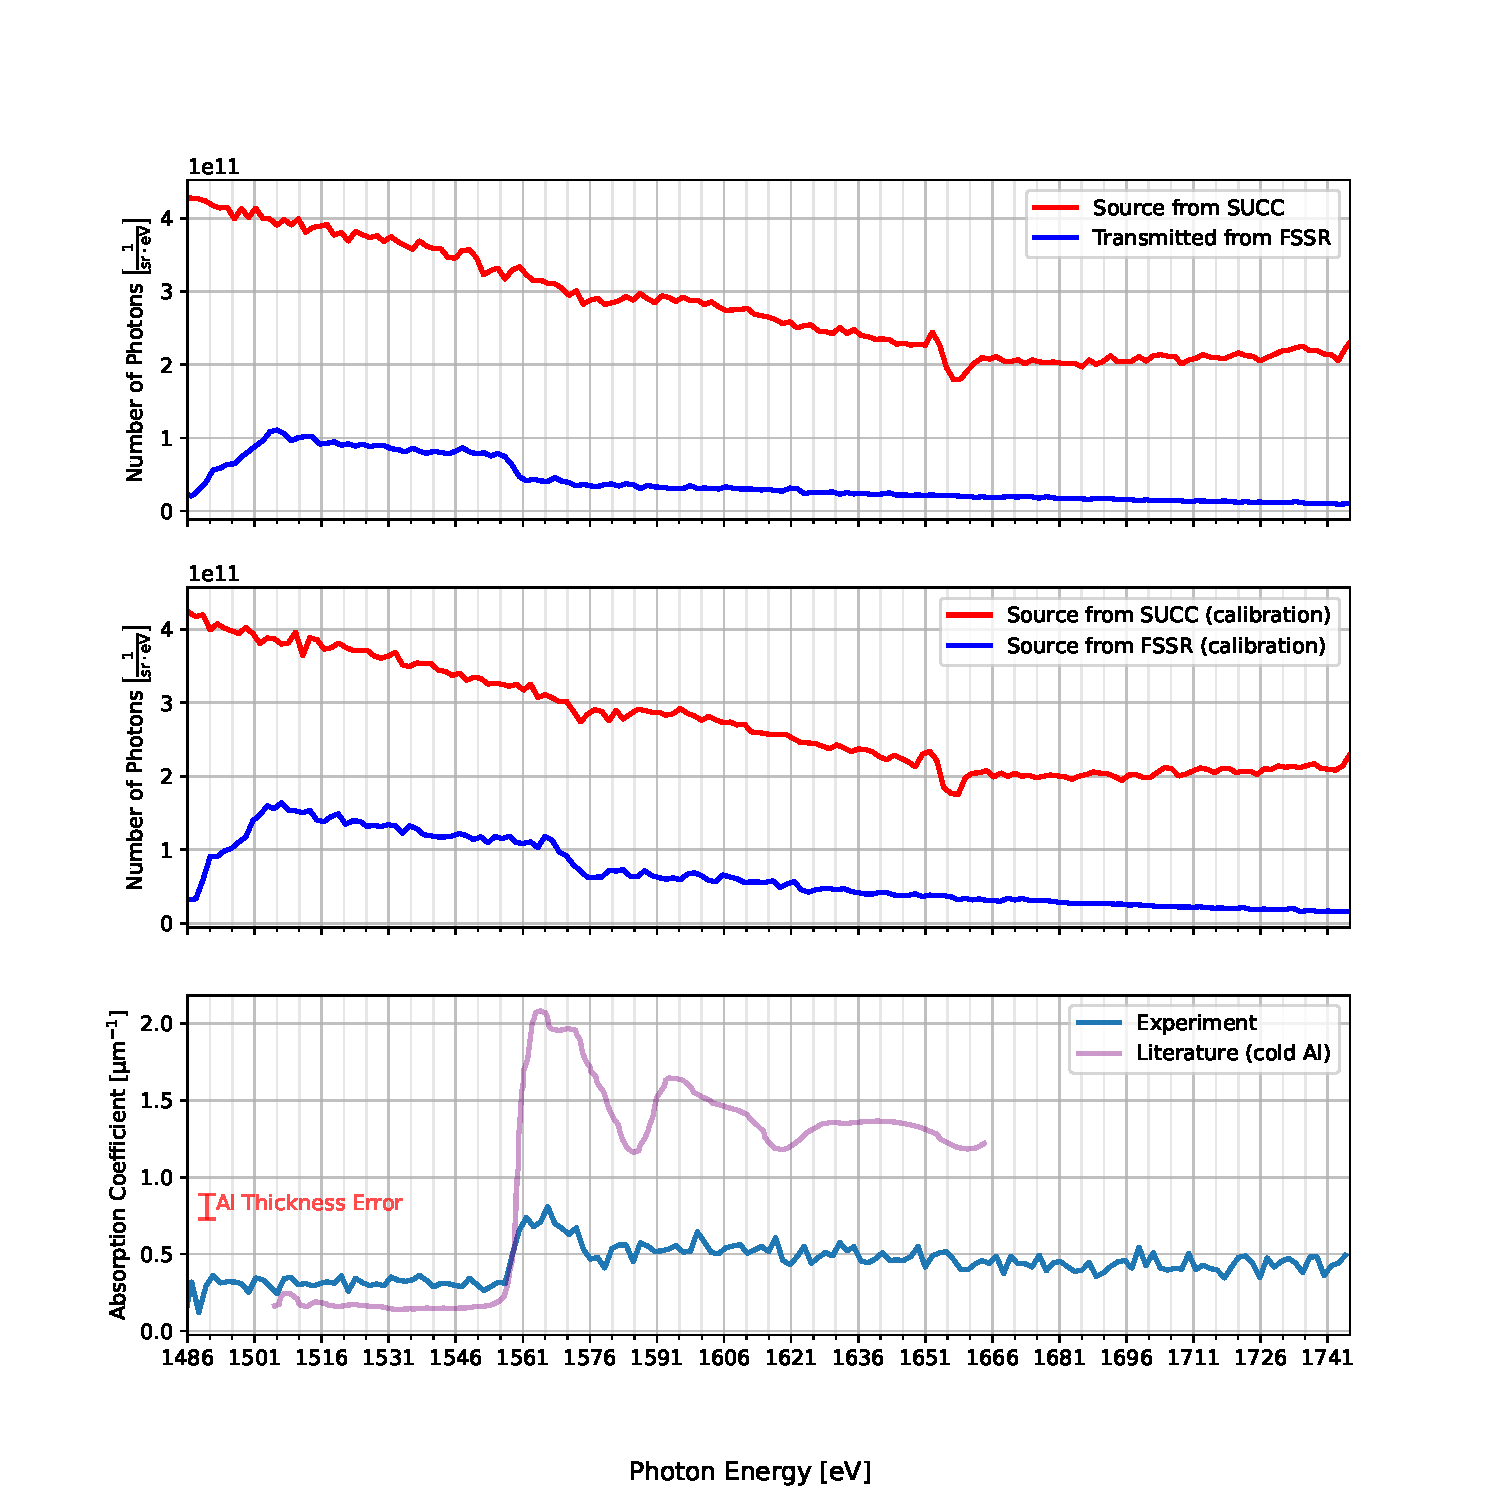
\includegraphics[width=\textwidth]{Data_Analysis/absorption/absorption_spectrum_of_PTFE_event_74_on_FSSR.pdf}
	\caption{X-ray absorption spectrum detected with the SUCC for the source and the FSSR for the transmitted spectrum. The crystal spectral features are corrected out using a calibration shot without a sample. \textbf{Top:} fully processed spectrum pair from a \SI{30.8}{\joule} shot on Teflon. The ratio of transmitted to source spectrum along with the crystal calibration yields the x-ray transmission through a \SI{1.0\pm0.1}{\micro\meter} thick aluminum foil sample. \textbf{Middle:} fully processed calibration spectrum pair from a \SI{30.4}{\joule} shot on Teflon. \textbf{Bottom:} absorption spectrum with comparison to a result from \textit{Levy et al.} \citep{levy2010double} and the systematic uncertainty due to the sample thickness, depicted as an error bar that aligns with the maximum value of $\mu$.}
	\label{fig: FSSR absorption}
\end{figure}


\section{Spectrometer Characterization}
\label{section: spectrometer characterization}

To perform a quantitative analysis of the spectrometer performance, properties of three spectrometers, namely the DUCC, FSSR, and SUCC, will be investigated, giving insight into the extent to which the designs were successfully implemented. First, I will calculate the ratio of the integrated reflectivities of the crystals for each spectrometer pairing, as well as infer the $R_{int}$ value of the mica crystal in the FSSR with the help of a simulation carried out by Artem Martynenko, allowing further characterization of the crystals and assessment of their impact on the spectrometers' performance. Second, the spectral resolution and its contributions will be determined for all the spectrometers using the He-$\upalpha$ line emission of aluminum, along with the steepness of the K-edge in transmission spectra of Al recorded with the DUCC. From these results, I will assess the efficacy of the \textit{mmpxrt} simulations and the viability of each spectrometer for its intended variant of XAFS.

In this section the crystal properties play a crucial role and therefore will be further elaborated on. As discussed in section \ref{section: resolution theory}, the relevant parameters are the integrated reflectivity $R_{int}$ and the rocking curve width $\Delta \theta$, which both are determined from a reflection curve at a given photon energy. $R_{int}$ parameterizes the reflectivity of the crystal, i.e. how many of the monochromatic photons are reflected, so that a larger $R_{int}$ implies a higher luminosity of the spectrometer, while $\Delta \theta$ gives the width of the reflection curve and impacts the spectral resolution of the spectrometer \citep{holzer1998flat}. In general, the more defects in a crystal the higher the integrated reflectivity and $\Delta \theta$. An important property of the integrated reflectivity is its independence from the x-ray source properties, like beam size, and shape of the reflection curve \citep{loisel2016measurement}. Because of this and the indirect relation of the two crystal properties, I will study $R_{int}$ and the spectral resolution separately.

Generally speaking, it is difficult to estimate $R_{int}$ and $\Delta \theta$ for a given crystal without directly measuring, since the quantities are highly sensitive to crystal quality, i.e. the density of crystal defects, and depend on the refraction order and photon energy \citep{ferrari2019characterization}, leading to significant variance among the literature. A good example of this is for ADP crystals, where integrated reflectivities can vary by an order of magnitude, as with the values \SI{2.32}{\micro\radian} \citep{ferrari2019characterization} and \SI{40}{\micro\radian} \citep{gilfrich1975integral}. Consequently, in section \ref{section: int refl ratio} the assumed values of the crystal properties will be adjusted according to new information gathered from Artem's simulation as well as experimental results, with which additional \textit{mmpxrt} simulations will be conducted and used to discuss the spectral resolutions of section \ref{subsection: spectral resolution}.

\subsection{Integrated Reflectivity Ratio}
\label{section: int refl ratio}

To build on the findings of the previous section, the ratio of $R_{int}$ between different crystals will now be determined, giving a deeper insight into the quality of the KAP, ADP, and mica crystals. I begin by extracting the source spectra of a shot on Al for two spectrometers, following the same process as described in chapter \ref{chapter: data analysis} but leaving out the binning and multiplying equation \ref{conversion to emitted photons} with $R_{int}$, $\Delta E$ and 4$\pi$. The quantity of interest becomes the integral over the $N_{\text{total}}\cdot R_{int}$ values for a given energy range, which I chose to cover the two emission lines at \SI{1588.3}{\electronvolt} and \SI{1598.4}{\electronvolt}, corresponding to the $n=2\rightarrow n=1$ transitions of heliumlike ions of aluminum \citep{thompson2001x}. An example of an integration area is given in fig. \ref{fig: R_int DUCC_t}, with the other cases available in the appendix section \ref{appendix: supplementary results}.\ref{appendix: integrated reflectivity ratio}. These lines are selected because they are the strongest that fall within the shared energy range of every spectrometer. The integral is approximated by summing, yielding
\begin{equation}
	\sum_{i}N_{\text{total}}(E_i)\cdot R_{int} = \frac{\sum_{i}[4\pi\cdot N_{\text{det}}(E_i)\cdot D(E_i)]}{\Delta x_{\text{pix}}},
	\label{eq: ratio of R_int}
\end{equation}
where as in chapter \ref{chapter: data analysis} $\Delta x_{\text{pix}}$ becomes $w_{\text{crystal}}$ for the FSSR. Next, by simply taking the ratio of the integral for both spectrometers of a shot, I can determine the integrated reflectivity ratio of the crystals. As previously noted, $R_{int}$ cannot be directly measured by this setup due to the unknown total number of emitted photons from the source $N_{\text{total}}$.

\begin{figure}[H]
	\centering
	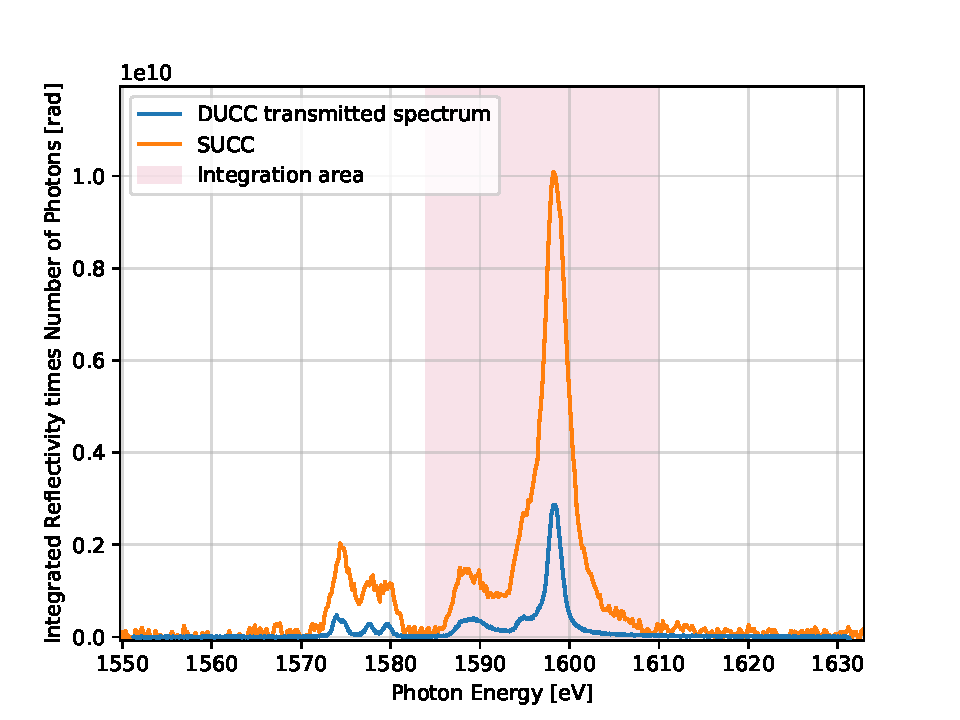
\includegraphics[width=0.8\textwidth]{Data_Analysis/R_int_ratio/spectra_of_Al_event_19_transmitted.pdf}
	\caption{$R_{int}\cdot N_\text{{total}}$ for a \SI{27}{\joule} shot on aluminum (event 19). The spectra from the transmission channel of the DUCC and the SUCC are presented, as well as the integration area used to calculate the integrated reflectivity ratio.}
	\label{fig: R_int DUCC_t}
\end{figure}

In addition to the method above, the $R_{int}$ for the mica crystal of the FSSR will be calculated directly by using the efficiency $\gamma$ of the FSSR spectrometer with mica crystal, derived in a simulation conducted by Artem Martynenko using the parameters of the FSSR geometry of this work and mica crystals typical of Sergey Pikuz' lab, where the crystal of this experiment originates. The efficiency is defined as the ratio the simulated photons reaching the detector $N_{\text{det,sim}}$ and the total number of emitted photons $N_{\text{total,sim}}$, i.e. $N_{\text{det,sim}}/N_{\text{total,sim}}$. I determine the integrated reflectivity of the FSSR by first linearly interpolating the efficiency data of fig. \ref{fig: efficiency graph} to get $\gamma(E)$. Then, equation \ref{eq: ratio of R_int} is applied to derive
\begin{equation}
	R_{int} = \frac{\sum_{i}[4\pi\cdot N_{\text{det}}(E_i)\cdot D(E_i)]/w_{\text{crystal}}}{\sum_{j}(N_{\text{det}}(E_j)/\gamma(E_j))},
\end{equation}
where the summations are over the same energy range described in the first method.



\begin{figure}[H]
	\centering
	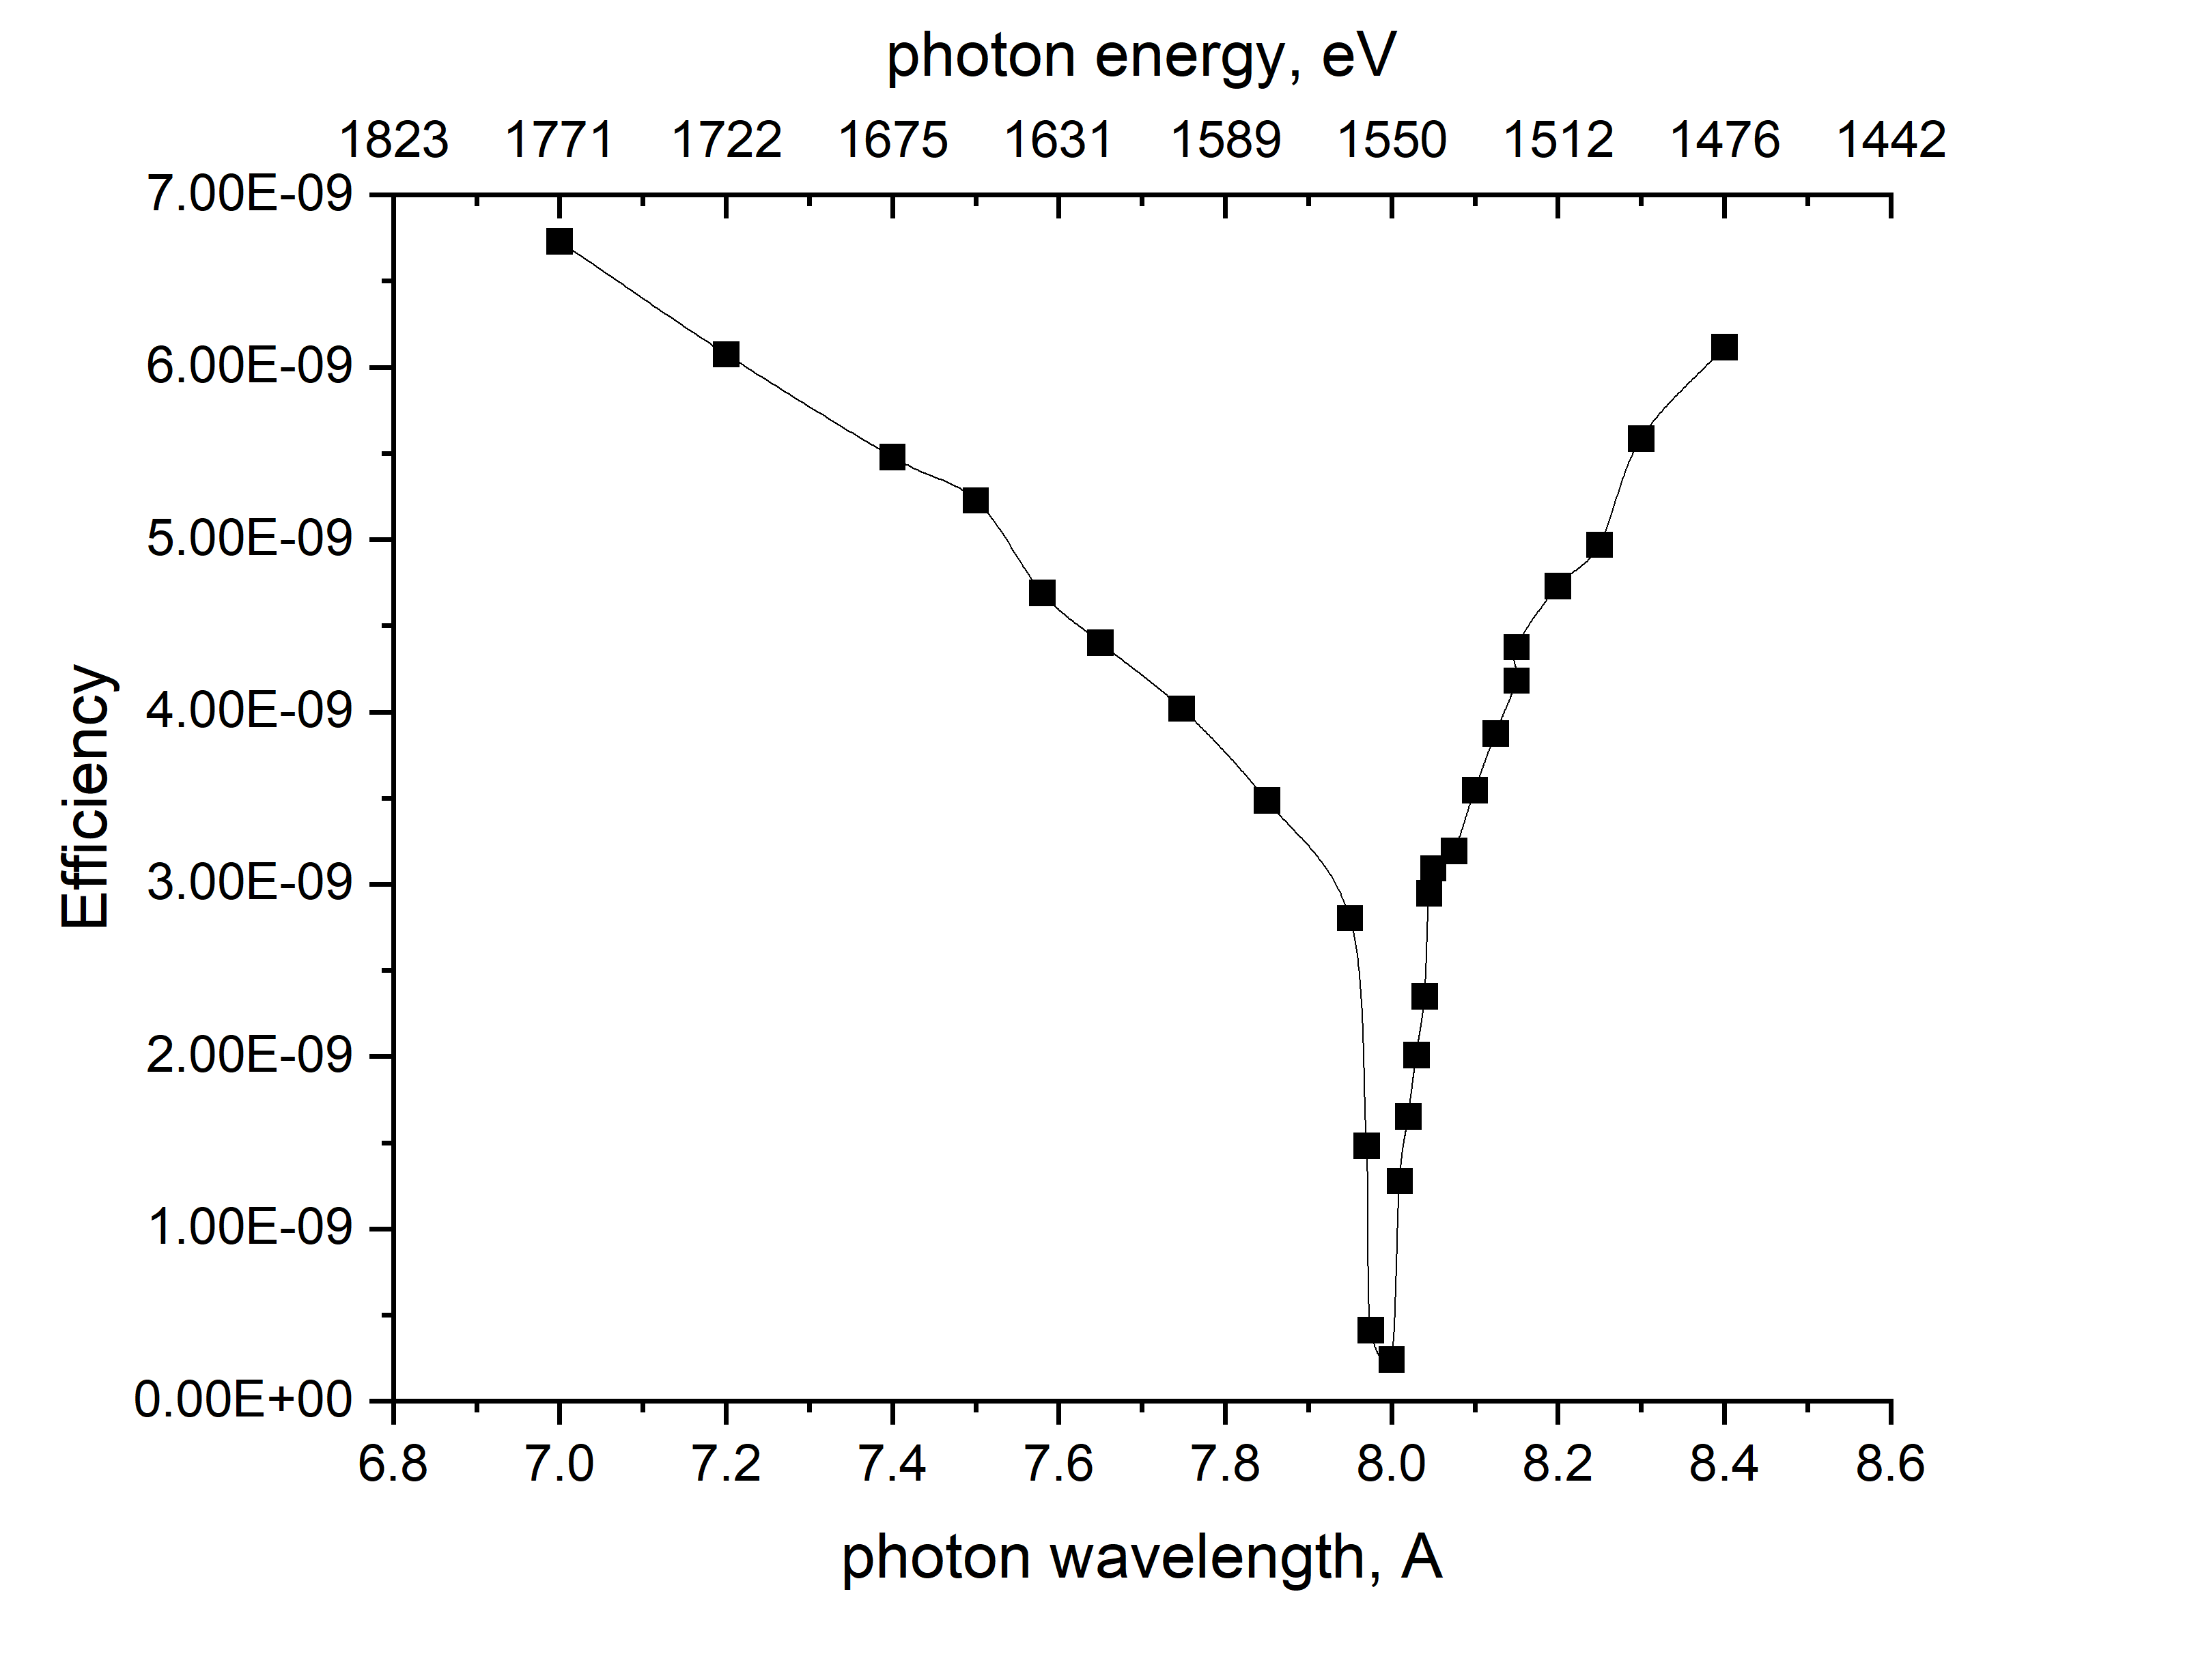
\includegraphics[width=0.8\textwidth]{Data_Analysis/efficiency_graph.png}
	\caption{Efficiency of the FSSR-1D with a mica crystal typical of Sergey Pikuz' lab, extracted by a ray tracing simulation carried out by Artem Martynenko. Immediately recognizable is a dip around 1540-\SI{1560}{\electronvolt}, which is related to the K-edge of the aluminum component of the mica crystal.}
	\label{fig: efficiency graph}
\end{figure}

The results will be compared to the estimated literature values for $R_{int}$ of \SI{40}{\micro\radian} for the ADP crystals of the DUCC \citep{gilfrich1975integral}, \SI{80}{\micro\radian} for the KAP crystal of the SUCC \citep{loisel2016measurement}, and \SI{53.6}{\micro\radian} for the mica crystal of the FSSR \citep{holzer1998flat}. In this case, \SI{40}{\micro\radian} is chosen over the value of \SI{2.32}{\micro\radian} used in the \textit{mmpxrt} simulations of section \ref{section: specs and comparison} because it lies closer to the experimental results in table \ref{Table: Rint Ratio}.

The results in table \ref{Table: Rint Ratio} for the experimentally determined ratios of the DUCC to the SUCC lie close to 1 and deviate from the expected values by less than a factor of 2, indicating that the ADP crystals have a $R_{int}$ larger than the literature value, the KAP crystals of the SUCC exhibit a lower integrated reflectivity, or some combination of the two. Interestingly, this also points to the ADP and KAP crystals having comparable integrated reflectivities, from which one would intuitively expect that the signal intensities on detector be similar, but the fact that the signal-to-noise ratio of the teflon backlighter/DUCC combination is too low to be feasible refutes this expectation. The difference between the photon intensity on the DUCC and SUCC can be explained by the difference in energy range, where the DUCC collects photons on more pixels for a given energy interval than the SUCC, reducing the overall photon count per pixel. Another interesting observation is that the DUCC/SUCC ratios for each channel of the DUCC are unequal, implying that the integrated reflectivity of each ADP crystal is different. This highlights the crystal-to-crystal variance in properties, even when they share an origin and fabrication process.

In contrast to the DUCC/SUCC ratios, the experimental FSSR/SUCC ratio of $0.062\pm0.015$ is around a factor of 10 smaller than the literature value. As the DUCC/SUCC ratios do not deviate so significantly, the discrepancy for the FSSR is likely due to the actual integrated reflectivity of the mica crystal being significantly lower than the literature value of \SI{53.6}{\micro\radian}. Further insight is offered by inferring a $R_{int}$ for mica using the simulated efficiency $\gamma$, which with the method described previously yields a value of \SI{2.752\pm0.633}{\micro\radian}, an order of magnitude lower than that of the literature. Accordingly, the $R_{int}$ from the simulation is in better agreement with the experimental FSSR/SUCC ratio. With the simulated $R_{int}$ of the mica crystal and the experimental ratios, new integrated reflectivities can be extracted for the crystals of the DUCC and SUCC. Inserting the new $R_{int}$ value into the experimental ratio FSSR/SUCC and propagating the uncertainties yields an integrated reflectivity of \SI{44.39\pm14.82}{\micro\radian} for the SUCC. Repeating this process again for the DUCC results in \SI{37.13\pm11.98}{\micro\radian}. 


\begin{table}[H]
	\centering
	\caption{Ratio of $R_{int}$ for various spectrometer combinations. DUCC$_t$ refers to the transmission channel of the DUCC and DUCC$_s$ to the source channel. The literature ratios are calculated using \SI{40}{\micro\radian} for the DUCC, \SI{80}{\micro\radian} for the SUCC, and \SI{53.6}{\micro\radian} for the FSSR.}
	\vspace{0.05cm}
	\renewcommand{\arraystretch}{1.5}
	\centering
	\begin{tabular}{|c|c|c|c|c|} 
		\hline
		Event & Shot & Spectrometer & Literature Ratio & Experimental Ratio \\ 
		[0.5ex]
		\hline\hline
		19 & \SI{27}{\joule} on Al & DUCC$_t$/SUCC & 0.5 & 0.892$\pm$0.047 \\ 
		[0.5ex]
		\hline
		19 & \SI{27}{\joule} on Al & DUCC$_s$/SUCC & 0.5 & 0.781$\pm$0.041 \\ 
		[0.5ex]
		\hline
		16 & \SI{24}{\joule} on Al & FSSR/SUCC & 0.67 & 0.062$\pm$0.015 \\ 
		[0.5ex]
		\hline
	\end{tabular}
	\label{Table: Rint Ratio}
\end{table}

Based on these results it is clear that the crystal properties used in the original \textit{mmpxrt} simulations during the design stage need to be adjusted in order to check the theoretical spectral resolution results of section \ref{section: specs and comparison}. As such, new \textit{mmpxrt} simulations are conducted for the DUCC and FSSR, whose results are given in the appendix section \ref{appendix: supplementary results}.\ref{section: new simulations}. The new DUCC simulation uses an integrated reflectivity of \SI{40}{\micro\radian} (originally \SI{2.32}{\micro\radian}). This higher $R_{int}$ yields more reflected rays in the simulation, enabling the use of the literature rocking curve width of \SI{165}{\micro\radian} \citep{rajesh2015growth}. These parameters give a spectral resolution of \SI{0.685}{\electronvolt}, approximately aligning with the original value of \SI{0.703}{\electronvolt} that contained an analytical estimate of the broadening due to crystal properties (see appendix section \ref{section: all simulations}.\ref{section: DUCC Simulation}). Due to this agreement, the original values in table \ref{TableResolutions} will be used in the following section. As for the FSSR, the new simulation uses the $R_{int}$ of \SI{2.752}{\micro\radian} as determined from the simulated efficiency. The rocking curve width is changed to \SI{349}{\micro\radian}, which was also delivered by Artem's simulation. The new parameters yield a $\Delta E$ of \SI{0.563}{\electronvolt}, significantly better than the value of \SI{3.097}{\electronvolt} of the design phase. Since the simulated $R_{int}$ value agrees more closely to the experimental FSSR/SUCC ratio, the results of the new FSSR simulation will be used for the further discussion. 


\subsection{Spectral Resolution}
\label{subsection: spectral resolution}

The analysis of the spectral resolution begins with the extraction of spectra, following the same method as chapter \ref{chapter: data analysis} except for not binning the data in order to maximize the number of data points. In the case of the calculations using the He-$\upalpha$ line, the peak at \SI{1598.4}{\electronvolt} in aluminum source spectra is first isolated. Due to the influence of a neighboring small emission line (see fig. \ref{fig: Al DUCC series}), the data is cut at the lower energy side of the peak where the photon numbers are below the half maximum. The empty region is then replaced by mirroring the higher energy side of the line, taking only the photon numbers with values below half the maximum. Consequently, a near symmetrical, approximately Gaussian peak remains. The data points are then fitted to a Gaussian function of the form
\begin{equation}
	N_{\text{st,eV}}(E_{\text{ph}}) = A\cdot \exp\left(\frac{-(E_{\text{ph}}-\mu)^2}{2\sigma^2}\right)+c
\end{equation}
with the fit parameters $A$, $\mu$, $\sigma$, and $c$. The goal is to determine the FWHM through the equation
\begin{equation}
	\text{FWHM} = 2\sqrt{2\ln(2)}\cdot \sigma,
\end{equation}
corresponding to the convolution of a number of line broadening mechanisms. The significant contributions are Doppler broadening due to the thermal motion of the ions in the plasma and spectrometer resolution (see section \ref{section: resolution theory}), consisting of source broadening, detector resolution, and broadening due to crystal properties, the latter henceforth referred to as crystal broadening, which is affected by geometry as well as crystal quality. The spectrometer resolution is directly relevant to the absorption spectra for XAFS, while the Doppler broadening is an aspect of the emission line used here. Assuming that each contribution has a Gaussian distribution, I calculate the crystal broadening $\sigma_{\text{crystal}}$ by deconvolving the FHWM result with 
\begin{equation}
	\sigma_{\text{crystal}} = \sqrt{\text{FWHM}^2-\sum_{i}^{n}\sigma_i^2},
	\label{eq: crystal broadening}
\end{equation}
where the sum over $\sigma_i$ represents the resolution contributions listed above apart from the crystal broadening. By comparing $\sigma_{\text{crystal}}$ to the results of the \textit{mmpxrt} simulations, I will assess the spectrometer performance and quality of the crystals.

In the case of the DUCC, the resolution can also be found using the transmission $T$ from absorption shots. This method leverages the dual channel aspect of the geometry and the absence of significant crystal features in the spectra and works under the assumption that the resolutions of both channels are equal. For the analysis I first extract the transmission spectrum analogously to the method described in section \ref{subsection: ab spectra}. Next, I fit the data with the modified error function
\begin{equation}
	N_{\text{st,eV}}(E_{\text{ph}}) = A\cdot\text{erf}\left(\frac{-(E_{\text{ph}}-\mu)}{(\sigma\sqrt{2})}\right)+c \quad\text{with}\quad \text{erf}(z) = \frac{2}{\sqrt{\pi}}\int_{0}^{z}e^{-t^2}dt,
\end{equation}
yielding the same fit parameters as with the Gaussian function. Finally, $\sigma_{\text{crystal}}$ can be determined just as with the He-$\upalpha$ line, except without the Doppler broadening contribution.

In order to have full insight into the FWHM uncertainty calculation, I conduct the fitting with a self-built algorithm that tests a range of possible FWHM values. The algorithm functions as follows:
\begin{enumerate}
	\item Initialize a set of evenly spaced FWHM values ranging from 0.5-\SI{7}{\electronvolt}.
	\item Loop through the FWHM set, where for each value a model is created by fitting the data while holding the fit parameter $\sigma$ constant as calculated from the FWHM.
	\item The "goodness" of each model is parameterized using the reduced chi-squared test, which determines a $\chi^2$ value with the formula
	\begin{equation}
		\chi^2 = \frac{1}{n-m}\sum_{i}^{n}\frac{(O_i-M_i)^2}{s_i^2},
	\end{equation}
	where $O_i$ is the observed data point, $M_i$ the corresponding fitted value, $s_i$ the statistical error of the data point, $n$ the number of data points, and $m$ the number of fit parameters.
	\item With this test, models are generally accepted if $\chi^2\leq 1$. In this case, the error of the data used for the resolution calculation, consisting of purely statistical error from the camera and Poisson noise, and the Gaussian fit result in a $\chi^2 > 1$ for all spectrometers. This is attributed to two different effects: the error is incorrect, giving a too small uncertainty relative to the data, and/or the model does not accurately represent the data, a possibility that will be discussed later. Since I only want to determine the FWHM, I consider a model acceptable if $\chi^2\leq1.5\cdot\chi^2_{min}$, where $\chi^2_{min}$ is defined as the minimum value of all the fit models. I chose the prefactor 1.5 heuristically by testing the fits and gradually reducing the prefactor until the fringe models were visually reasonable.
	\item The final FWHM is chosen from the best model, i.e. with $\chi^2_{min}$. The bounds of the error are given by the absolute difference between the best FWHM and the worst accepted FWHM, so with the largest $\chi^2$ within the accepted range.
\end{enumerate}
In the following I present the fits of data produced by the algorithm for the DUCC, FSSR, and SUCC. The graphs of the remaining shots not shown can be found in the appendix section \ref{appendix: supplementary results}.\ref{appendix: spectral resolution}.

\begin{figure}[H]
	\centering
	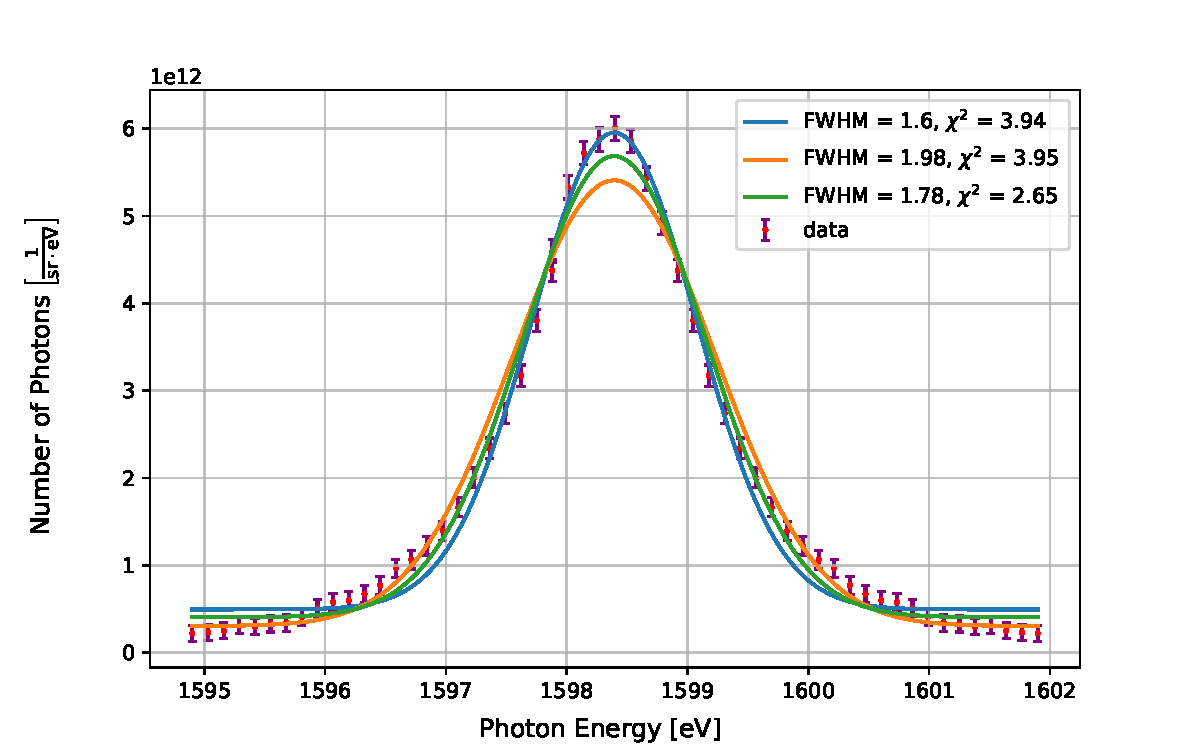
\includegraphics[width=0.9\textwidth]{Data_Analysis/resolution/peak_of_Al_(thick)_event_16_on_FSSR.pdf}
	\caption{Gaussian fit of the He-$\upalpha$ line for a \SI{24}{\joule} shot on aluminum (event 16) used to determine the spectral resolution of the FSSR. The best (green) and worst (blue and orange) fit models are depicted and labeled with their corresponding FWHM and $\chi^2$ values.}
	\label{fig: resolution FSSR}
\end{figure}

\begin{figure} [H]
	\centering
	\begin{subfigure}[t]{0.9\textwidth}
		\centering
		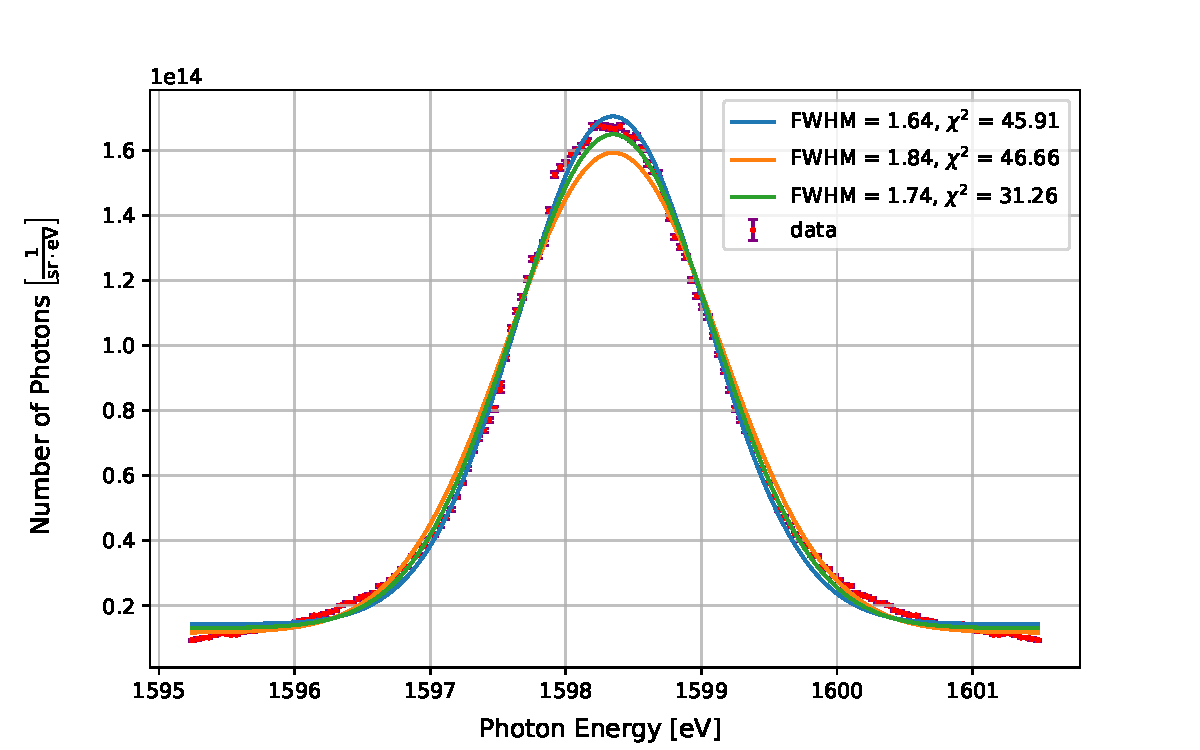
\includegraphics[width=\textwidth]{Data_Analysis/resolution/peak_of_Al_event_19_on_DUCC.pdf}
		\caption{Gaussian fit of the He-$\upalpha$ line for a \SI{27}{\joule} shot on aluminum (event 19).}
		\label{}
	\end{subfigure}%
	\hfill
	\begin{subfigure}[t]{0.9\textwidth}
		\centering
		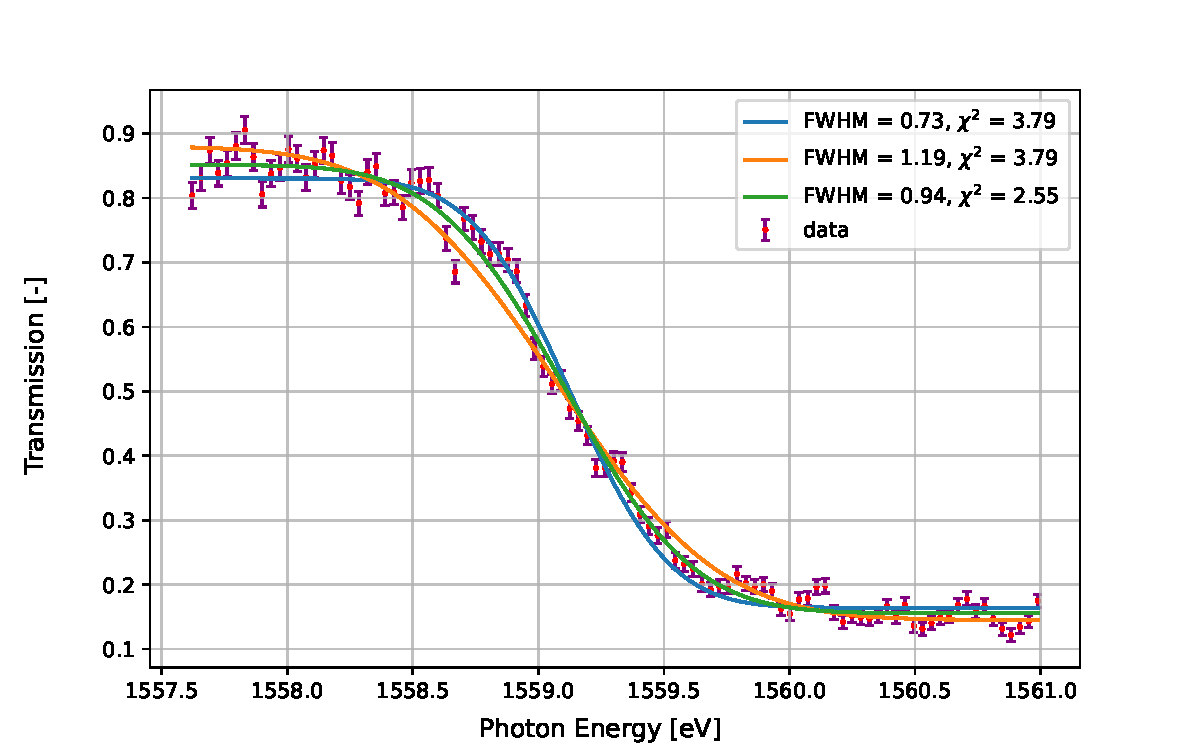
\includegraphics[width=\textwidth]{Data_Analysis/resolution/transmission_of_Gd_event_32_on_DUCC.pdf}
		\caption{Error function fit of the transmission through a \SI{1.18\pm0.12}{\milli\meter} thick aluminum sample for a \SI{87.4}{\joule} shot on gadolinium (event 32).}
		\label{}
	\end{subfigure}
	\caption{Fits used to determine the spectral resolution of the DUCC with a (a) Gaussian fit and (b) error function fit respectively. The best (green) and worst (blue and orange) fit models are depicted and labeled with their corresponding FWHM and $\chi^2$ values.}
	\label{}
\end{figure}

\begin{figure}[H]
	\centering
	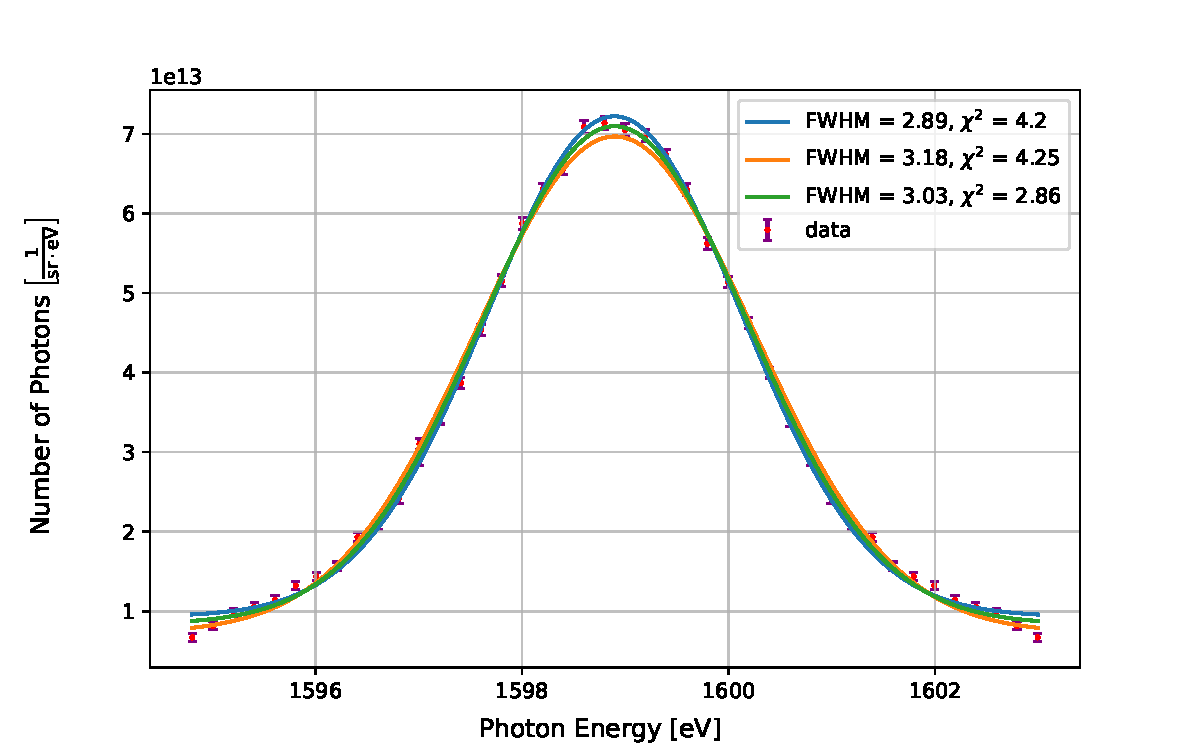
\includegraphics[width=0.9\textwidth]{Data_Analysis/resolution/peak_of_Al_event_18_on_SUCC.pdf}
	\caption{Gaussian fit of the He-$\upalpha$ line for a \SI{28}{\joule} shot on aluminum (event 18) used to determine the spectral resolution of the SUCC. The best (green) and worst (blue and orange) fit models are depicted and labeled with their corresponding FWHM and $\chi^2$ values.}
	\label{}
\end{figure}

For the SUCC and DUCC the source broadening plays a crucial role. It is derived from the source size and is influenced by the spectrometer geometry. To determine the source size, we placed a knife edge on the SUCC, consisting of an opaque metal sheet placed in front of the crystal in the x-ray path in such a way as to cover approximately half of the source image on the detector. By fitting an error function to the edge of the shadow cast by the knife edge and taking into account the magnification of the image, the FWHM of the source size in non-dispersive direction can be extracted. I then begin calculating the source broadening by projecting the source size $x_s$ onto the detector of a given spectrometer with the formula
\begin{equation}
	x_{s,d} = \frac{x_s}{\cos(\theta_0)}.
\end{equation}
The source image size $x_{s,d}$ is converted to eV using the dispersion of the spectrometer, finally resulting in the source broadening. To note is that all shots used to calculate the resolution using transmission were with a phase plate, while all the shots using the He-$\upalpha$ emission line were without a phase plate.

The Doppler broadening is from a FLYCHK simulation with the electron temperature $T_e$ = \SI{1000}{\electronvolt}, whose error is estimated from comparison to a simulation of $T_e$ = \SI{500}{\electronvolt}. In both simulations the electron density is set to \SI{4e21}{\centi\meter}$^{-3}$.

In the following I present the results for the spectral resolution calculations of the DUCC, FSSR, and SUCC. The final results for the crystal broadening as compared to the \textit{mmpxrt} simulations, adjusted according to the discussion of section \ref{section: int refl ratio}, are then given. 

The results for the DUCC shown in table \ref{Table: DUCC resolution} are calculated by neglecting the detector resolution contribution to the spectral resolution, a property that is apparent in table \ref{TableResolutions}. Interestingly, all the source sizes are larger than \SI{120}{\micro\meter} across different backlighter materials, which is expected for event 31 and 32 due to the use of a phase plate with a focus spot of at least \SI{120}{\micro\meter} in size, supporting the effectiveness of the knife edge method. Further investigation of the source sizes of a wider range of shots could be instructive for the optimization of the backlighter in future experiments. Furthermore, it is clear that the crystal broadening is the dominant contribution for the DUCC, in contrast to the theoretical predictions, where the source broadening was most significant. The higher than expected crystal broadening points to a high rocking curve width of the crystals and therefore worse crystal quality, which could be due to the fact that the ADP crystals were left exposed to air for a long period of time, as all the crystals were packaged together. The exposure could have caused absorption of water in the crystal, altering the lattice structure and crystal properties. Additionally, the crystal broadening values calculated from the transmission are in agreement, in the sense that they fall within each other's uncertainty, allowing the averaging of the two values to get $\left(0.94^{+0.31}_{-0.22}\right)$ eV. The large error range as compared to the Gaussian fit result can be attributed to the propagation of the error of two spectra, from which the transmission is determined. The crystal broadening from the transmission is more than \SI{0.6}{\electronvolt} lower than that from the Gaussian fit, a deviation that will be discussed later in this section. 

\begin{table}[H]
	\centering
	\caption{Resolution contributions of the DUCC calculated for different shots, where every value is given in eV unless another unit is expressly assigned. The results are obtained by a Gaussian fit to the Al He-a line (g) or an error function fit to the transmission (t). The detector resolution of the DUCC is negligible (see table \ref{TableResolutions}) and therefore not shown.}
	\vspace{0.05cm}
	\renewcommand{\arraystretch}{1.5}
	\centering
	\begin{tabular}{|c|c|c|c|c|c|c|c|} 
		\hline
		Event & Shot & Type & FWHM & \makecell{Source Size \\ $[$mm$]$} & \makecell{Source \\ Broadening} & \makecell{Doppler \\ Broadening} & \makecell{Crystal \\ Broadening} \\ 
		[0.5ex]
		\hline\hline
		19 & \SI{27}{\joule} on Al & g & 1.74$^{+0.11}_{-0.01}$ & 0.12$\pm$0.02 & 0.49$\pm$0.06 & 0.47$\pm$0.10 & 
		1.60$^{+0.12}_{-0.11}$ \\ 
		[0.5ex]
		\hline
		31 & \SI{92.7}{\joule} on Sm & t & 1.29$^{+0.47}_{-0.32}$ & 0.15$\pm$0.002 & 0.61$\pm$0.01 & - & 
		1.13$^{+0.53}_{-0.36}$ \\ 
		[0.5ex]
		\hline
		32 & \SI{87.4}{\joule} on Gd & t & 0.94$^{+0.25}_{-0.21}$ & 0.14$\pm$0.002 & 0.57$\pm$0.01 & - & 
		0.75$^{+0.32}_{-0.26}$ \\  
		[0.5ex]
		\hline
	\end{tabular}
	\label{Table: DUCC resolution}
\end{table}

In the case of the FSSR, the source broadening becomes negligible thanks to the focusing properties of the geometry, while the detector resolution is relevant. As displayed in table \ref{Table: FSSR resolution}, the main contribution to the spectral resolution is crystal broadening, where both shots yield approximately \SI{1.7\pm0.2}{\electronvolt}. The excellent agreement, despite the difference in laser energy of more than a factor 10, speaks for the efficacy of the analysis procedure. That the crystal broadening dominates is in agreement with theory.

\begin{table}[H]
	\centering
	\caption{Resolution contributions of the FSSR calculated for different shots, where every value is given in eV unless another unit is expressly assigned. The results are obtained by a Gaussian fit to the Al He-a line (g). The source broadening is negligible due to the focusing properties of the FSSR (see table \ref{TableResolutions}). The detector resolution uncertainty is neglected, as it is small compared to other error sources because of the precisely known pixel size.}
	\vspace{0.05cm}
	\renewcommand{\arraystretch}{1.5}
	\centering
	\begin{tabular}{|c|c|c|c|c|c|c|} 
		\hline
		Event & Shot & Type & FWHM & \makecell{Detector \\ Resolution} & \makecell{Doppler \\ Broadening} & \makecell{Crystal \\ Broadening} \\ 
		[0.5ex]
		\hline\hline
		2 & \SI{1.7}{\joule} on Al & g & 1.80$^{+0.19}_{-0.18}$ & 0.14 & 0.47$\pm$0.10 & 
		1.73$^{+0.20}_{-0.19}$ \\ 
		[0.5ex]
		\hline
		16 & \SI{24}{\joule} on Al & g & 1.78$^{+0.20}_{-0.18}$ & 0.14 & 0.47$\pm$0.10 & 
		1.71$^{+0.21}_{-0.19}$ \\ 
		[0.5ex]
		\hline
	\end{tabular}
	\label{Table: FSSR resolution}
\end{table}

For the SUCC, the detector resolution is neglected, as the spectrometer shares a basic geometry with the DUCC. In table \ref{Table: SUCC resolution} the results are presented, where again the crystal broadening dominates. Most striking is that all the crystal broadening results are in good agreement, hovering around \SI{2.4}{\electronvolt}, although the FWHM values deviate by up to \SI{0.34}{\electronvolt}, falling outside the range of the errors of the FWHM. The FWHM discrepancy is compensated by the smaller source broadening of event 16, which indicates that the source broadening processing method functions well. The overall crystal broadening agreement across shots again shows that the resolution calculation method is reliable.

\begin{table}[H]
	\centering
	\caption{Resolution contributions of the SUCC calculated for different shots, where every value is given in eV unless another unit is expressly assigned. The results are obtained by a Gaussian fit to the Al He-a line (g). The detector resolution is assumed to be negligible, following from the shared basic design of the SUCC and DUCC.}
	\vspace{0.05cm}
	\renewcommand{\arraystretch}{1.5}
	\centering
	\begin{tabular}{|c|c|c|c|c|c|c|c|} 
		\hline
		Event & Shot & Type & FWHM & \makecell{Source Size \\ $[$mm$]$} & \makecell{Source \\ Broadening} & \makecell{Doppler \\ Broadening} & \makecell{Crystal \\ Broadening} \\ 
		[0.5ex]
		\hline\hline
		16 & \SI{24}{\joule} on Al & g & 2.69$^{+0.15}_{-0.14}$ & 0.08$\pm$0.01 & 1.16$\pm$0.20 & 0.47$\pm$0.10 & 
		2.38$^{+0.20}_{-0.19}$ \\ 
		[0.5ex]
		\hline
		18 & \SI{28}{\joule} on Al & g & 3.03$^{+0.15}_{-0.14}$ & 0.11$\pm$0.03 & 1.69$\pm$0.44 & 0.47$\pm$0.10 & 
		2.48$^{+0.35}_{-0.34}$ \\ 
		[0.5ex]
		\hline
		19 & \SI{27}{\joule} on Al & g & 2.92$^{+0.19}_{-0.18}$ & 0.11$\pm$0.02 & 1.69$\pm$0.33 & 0.47$\pm$0.10 & 
		2.34$^{+0.34}_{-0.33}$ \\ 
		[0.5ex]
		\hline
	\end{tabular}
	\label{Table: SUCC resolution}
\end{table}


\begin{table}[H]
	\centering
	\caption{The final results for the experimentally determined crystal broadening compared to simulation when applicable. The results are obtained by a Gaussian fit to the Al He-a line (g) or an error function fit to the transmission (t). The experimental broadening is calculated by the mean of the crystal broadening results of all available shots.}
	\vspace{0.05cm}
	\renewcommand{\arraystretch}{1.5}
	\centering
	\begin{tabular}{|c|c|c|c|} 
		\hline
		Spectrometer & Type & \makecell{Simulated \\ Broadening} & \makecell{Experimental \\ Broadening} \\ 
		[0.5ex]
		\hline\hline
		DUCC & g &  \SI{0.24}{\electronvolt} & $\left(1.60^{+0.12}_{-0.11}\right)$ eV \\ 
		[0.5ex]
		\hline
		DUCC & t & \SI{0.24}{\electronvolt} & $\left(0.94^{+0.31}_{-0.22}\right)$ eV \\ 
		[0.5ex]
		\hline
		FSSR & g & \SI{0.54}{\electronvolt} & $\left(1.72^{+0.15}_{-0.13}\right)$ eV \\ 
		[0.5ex]
		\hline
		SUCC & g & - & $\left(2.40^{+0.18}_{-0.17}\right)$ eV \\ 
		[0.5ex]
		\hline
	\end{tabular}
	\label{Table: Final Resolutions}
\end{table}

The considerations and adjustments of section \ref{section: int refl ratio} result in the following simulated crystal broadening: \SI{0.24}{\electronvolt} for the DUCC as in the design phase and \SI{0.54}{\electronvolt} for the FSSR as calculated by the deconvolution of the spectral resolution of the new \textit{mmpxrt} simulation from the detector resolution. Table \ref{Table: Final Resolutions} compares the simulated crystal broadening to the experimentally determined ones, where it is immediately apparent that the former deviate significantly from the latter. In all cases, the main cause likely lies in the discrepancy of the rocking curve widths used in the \textit{mmpxrt} simulations (\SI{349}{\micro\radian} for mica and \SI{165}{\micro\radian} for ADP) to the real, unmeasured values. This demonstrates the inherent difficulty in assuming accurate crystal properties purely from the literature. As such, a reasonable next step would be the direct measurement of the integrated reflectivity and rocking curve width of the crystals actually used/to be used in experiments. With this information, more accurate \textit{mmpxrt} simulations could be conducted, ensuring that the desired spectral resolution is achieved in experiment. Another interesting observation is the fact that all the experimental values are higher than the simulated ones. This is expected for the FSSR, whose $\Delta \theta$ of the simulation is determined from the ray tracing code of Artem, meaning that the rocking curve width of the actual crystal is increased due to defects or damage. Despite this, the experimental crystal broadening $\left(1.72^{+0.15}_{-0.13}\right)$ eV falls well below the result in the original \textit{mmpxrt} simulation of \SI{2.95}{\electronvolt} (see table \ref{TableResolutions}), implying that the mica crystal's quality is still significantly better than that calculated by \textit{Hölzer et al.} \citep{holzer1998flat}.

Another interesting finding from table \ref{Table: Final Resolutions} is the more than 50\% deviation of the crystal broadenings found with the transmission and the He-$\upalpha$ line for the DUCC, lying outside the margins of error. A possible origin of this discrepancy is additional broadening effects of the emission line which have not been accounted for, leading to an artificially inflated result for the He-$\upalpha$ line. The most probable mechanism is Stark broadening caused by interaction with charged particles in the plasma, which broadens lines according to a Lorentz distribution. Notably, Doppler broadening dominates for high electron temperature, low electron density plasma \citep{wiese1965plasma}, as is expected for the Al plasma where He-$\upalpha$ emission is the strongest. Still, the inherent spatial and temporal inhomogeneity of laser plasma means that the influence of the Stark broadening would have to be estimated with further simulations. Another indication that could point to Stark broadening is the form of the He-$\upalpha$ line, which the Gaussian fit does not entirely correspond to, as most easily seen in fig. \ref{fig: resolution FSSR}, but also apparent for all the spectrometers. The relatively far extending wings of the data are characteristic of the Lorentz profile \citep{kunze2009introduction} and indicate that the peak likely conforms to a Voigt profile, which is the convolution of the Gauss and Lorentz profile. Despite this, a Gaussian profile is applied for the fitting because it still closely describes the data and markedly simplifies the analysis, since the Voigt fitting would require an additional fitting parameter.

To close, the experimentally determined resolutions will be compared to the requirements for EXAFS and XANES respectively. The crystal broadening for the DUCC of $\left(1.60^{+0.12}_{-0.11}\right)$ eV using the Gaussian fit method and $\left(0.94^{+0.31}_{-0.22}\right)$ from the fit of the transmission combined with the source broadening both lie above the original spectrometer design consideration for conducting XANES of $\Delta E \leq\SI{1}{\electronvolt}$. Consequently, the future use of the DUCC geometry with ADP crystals requires that the crystal properties are measured beforehand and if necessary exchanged for new crystals. Conversely, the excellent spectral resolutions, as calculated by the deconvolution of the FWHM from the Doppler broadening, of $\left(1.72^{+0.15}_{-0.13}\right)$ eV for the FSSR and $\left(2.84^{+0.10}_{-0.09}\right)$ eV for the SUCC, easily fulfill the requirement of $\Delta E <\SI{10}{\electronvolt}$ for EXAFS. As such, both the spectrometers could be considered viable candidates for future designs, purely from a spectral resolution standpoint.


\section{Setup Validation}
\label{section: setup validation}

As of yet, the spectrometers, and by extension the experimental setup have been assessed without quantitative comparison to similar experiments. To remedy this and place the captured spectra in a broader context, the conversion efficiency of the PHELIX laser energy into the He-$\upalpha$ emission line of aluminum will be extracted. I will then check the reasonableness of the results by comparing them to the expected order of magnitude estimated from the literature. A more exacting comparison is not possible in this case due to the fundamental differences between experimental setups and studied backlighter materials.

\subsection{Conversion Efficiency into He-$\upalpha$ Emission Line of Aluminum}

I determine the conversion efficiency of the laser energy into the Al He-$\upalpha$ line by first processing the source spectra of shots on aluminum as described in chapter \ref{chapter: data analysis} without the binning step, where I use the same integrated reflectivity values from the literature as in section \ref{section: int refl ratio}. I then multiply the resulting $N_{\text{st,eV}}$ in equation \ref{conversion to emitted photons} with 4$\pi$ and $\Delta E$ to get the total number of emitted photons $N_{\text{total}}$ in each energy interval covered by a given pixel. Next, I approximate integrating by summing over all the energy intervals included in the He-$\upalpha$ line, avoiding the neighboring other heliumlike ion emission line. An example of an integration area is depicted in fig. \ref{fig: CE DUCC_t}. Multiplying the energy of the line, i.e. \SI{1598.4}{\electronvolt}, onto this sum yields the total energy emitted into the He-$\upalpha$ line. The ratio of this quantity to the laser energy then gives the desired conversion efficiency.

\begin{figure}[H]
	\centering
	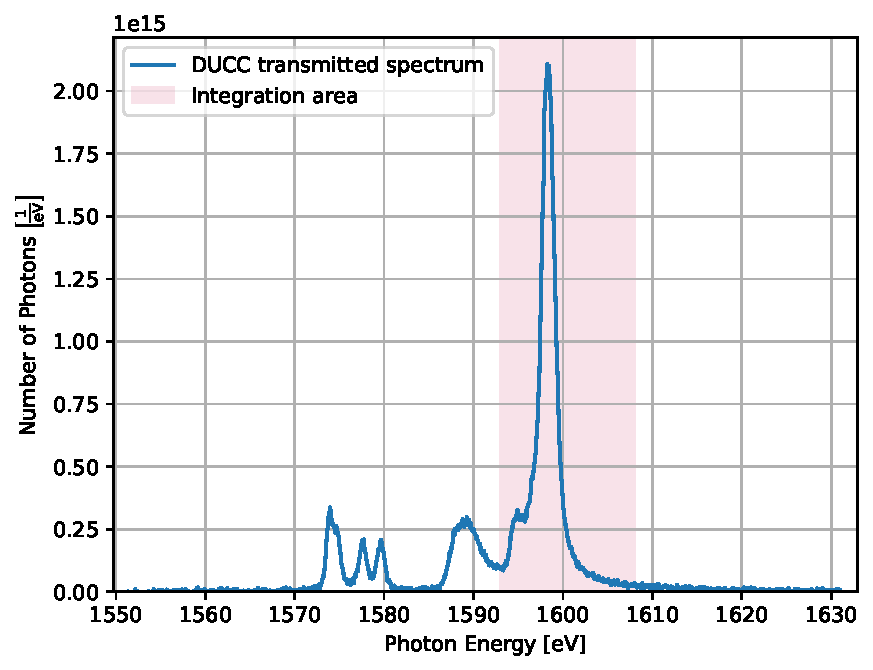
\includegraphics[width=0.8\textwidth]{Data_Analysis/converison_efficiency/spectra_of_Al_event_19_on_DUCC_transmitted_spectrum.pdf}
	\caption{Spectrum from a \SI{27}{\joule} shot on aluminum (event 19) captured with the transmission channel of the DUCC and utilized to determine the conversion efficiency. The area over which the data belonging to the Al He-$\upalpha$ line is summed is depicted in pink.}
	\label{fig: CE DUCC_t}
\end{figure}

As with the $R_{int}$ ratio, the conversion efficiency $CE$ using the FSSR can alternatively be determined through the simulated efficiency of the FSSR from section \ref{section: int refl ratio}. In this case, I use the $R_{int}$ of the mica crystal of \SI{2.752\pm0.633}{\micro\radian} derived in section \ref{section: int refl ratio} in place of the literature value and follow the same calculation as above.

In table \ref{Table: CE} I present the experimentally determined conversion efficiencies for each spectrometer, along with the integrated reflectivity used in the calculation. All the $CE$ are in the region of a few percent and lie approximately within each others error ranges, with the exception of the FSSR result derived using the literature $R_{int}$ value, again reinforcing the notion that the $R_{int}$ from simulation is closer to the actual value. This agreement also serves to demonstrate the consistency of the setup across all spectrometers and support the validity of the spectrum processing procedure.

\begin{table}[H]
	\centering
	\caption{Conversion efficiency of the laser energy into the He-$\upalpha$ line of aluminum. DUCC$_t$ refers to the transmission channel of the DUCC, DUCC$_s$ to the source channel. The integrated reflectivity value used in the calculation is given.}
	\vspace{0.05cm}
	\renewcommand{\arraystretch}{1.5}
	\centering
	\begin{tabular}{|c|c|c|c|c|} 
		\hline
		Event & Shot & Spectrometer & $R_{int}$ & \makecell{Conversion \\ Efficiency} \\ 
		[0.5ex]
		\hline\hline
		19 & \SI{27}{\joule} on Al & DUCC$_t$ & \SI{40}{\micro\radian} & (4.50$\pm$2.25)\% \\ 
		[0.5ex]
		\hline
		19 & \SI{27}{\joule} on Al & DUCC$_s$ & \SI{40}{\micro\radian} & (3.76$\pm$1.88)\% \\ 
		[0.5ex]
		\hline
		16 & \SI{24}{\joule} on Al & FSSR & \SI{53.6}{\micro\radian} & (0.20$\pm$0.10)\% \\ 
		[0.5ex]
		\hline
		16 & \SI{24}{\joule} on Al & FSSR & \SI{2.752}{\micro\radian} & (3.89$\pm$0.28)\% \\ 
		[0.5ex]
		\hline
		16 & \SI{24}{\joule} on Al & SUCC & \SI{80}{\micro\radian} & (2.55$\pm$1.28)\% \\ 
		[0.5ex]
		\hline
		19 & \SI{27}{\joule} on Al & SUCC & \SI{80}{\micro\radian} & (2.71$\pm$1.36)\% \\ 
		[0.5ex]
		\hline
	\end{tabular}
	\label{Table: CE}
\end{table}

For comparison, I estimate the expected order of magnitude for the results using values of the conversion efficiency of the Z-Beamlet laser at Sandia National Laboratories into He-like emission lines of laser-plasma of various elements ranging from Z$=21$ to 32 \citep{ruggles2003measurements}. Extrapolating from the conversion efficiencies in fig. 5 of \textit{Ruggles et. al.}'s paper, a $CE$ into the Al He-$\upalpha$ line on the order of 1\% is reasonable. Consequently, every spectrometer yields acceptable values, supporting the efficacy of the experimental setup as a whole.

